\author{Tadd\"aus Nauheimer}
\chapter{Step-by-Step Guide}

\section{How To}
Um die Software aufzurufen, einfach die Ihnen bereitgestellte URL in einem Browser \"offnen.
Anschließend kann diesem Guide weiter gefolgt werden.

\subsection{Frontpage und Dokument laden}

Hier ist die Frontpage der Software zu sehen.
Oben Links kann das erste Dokument geladen werden.

\begin{figure}[H]
    \centering
    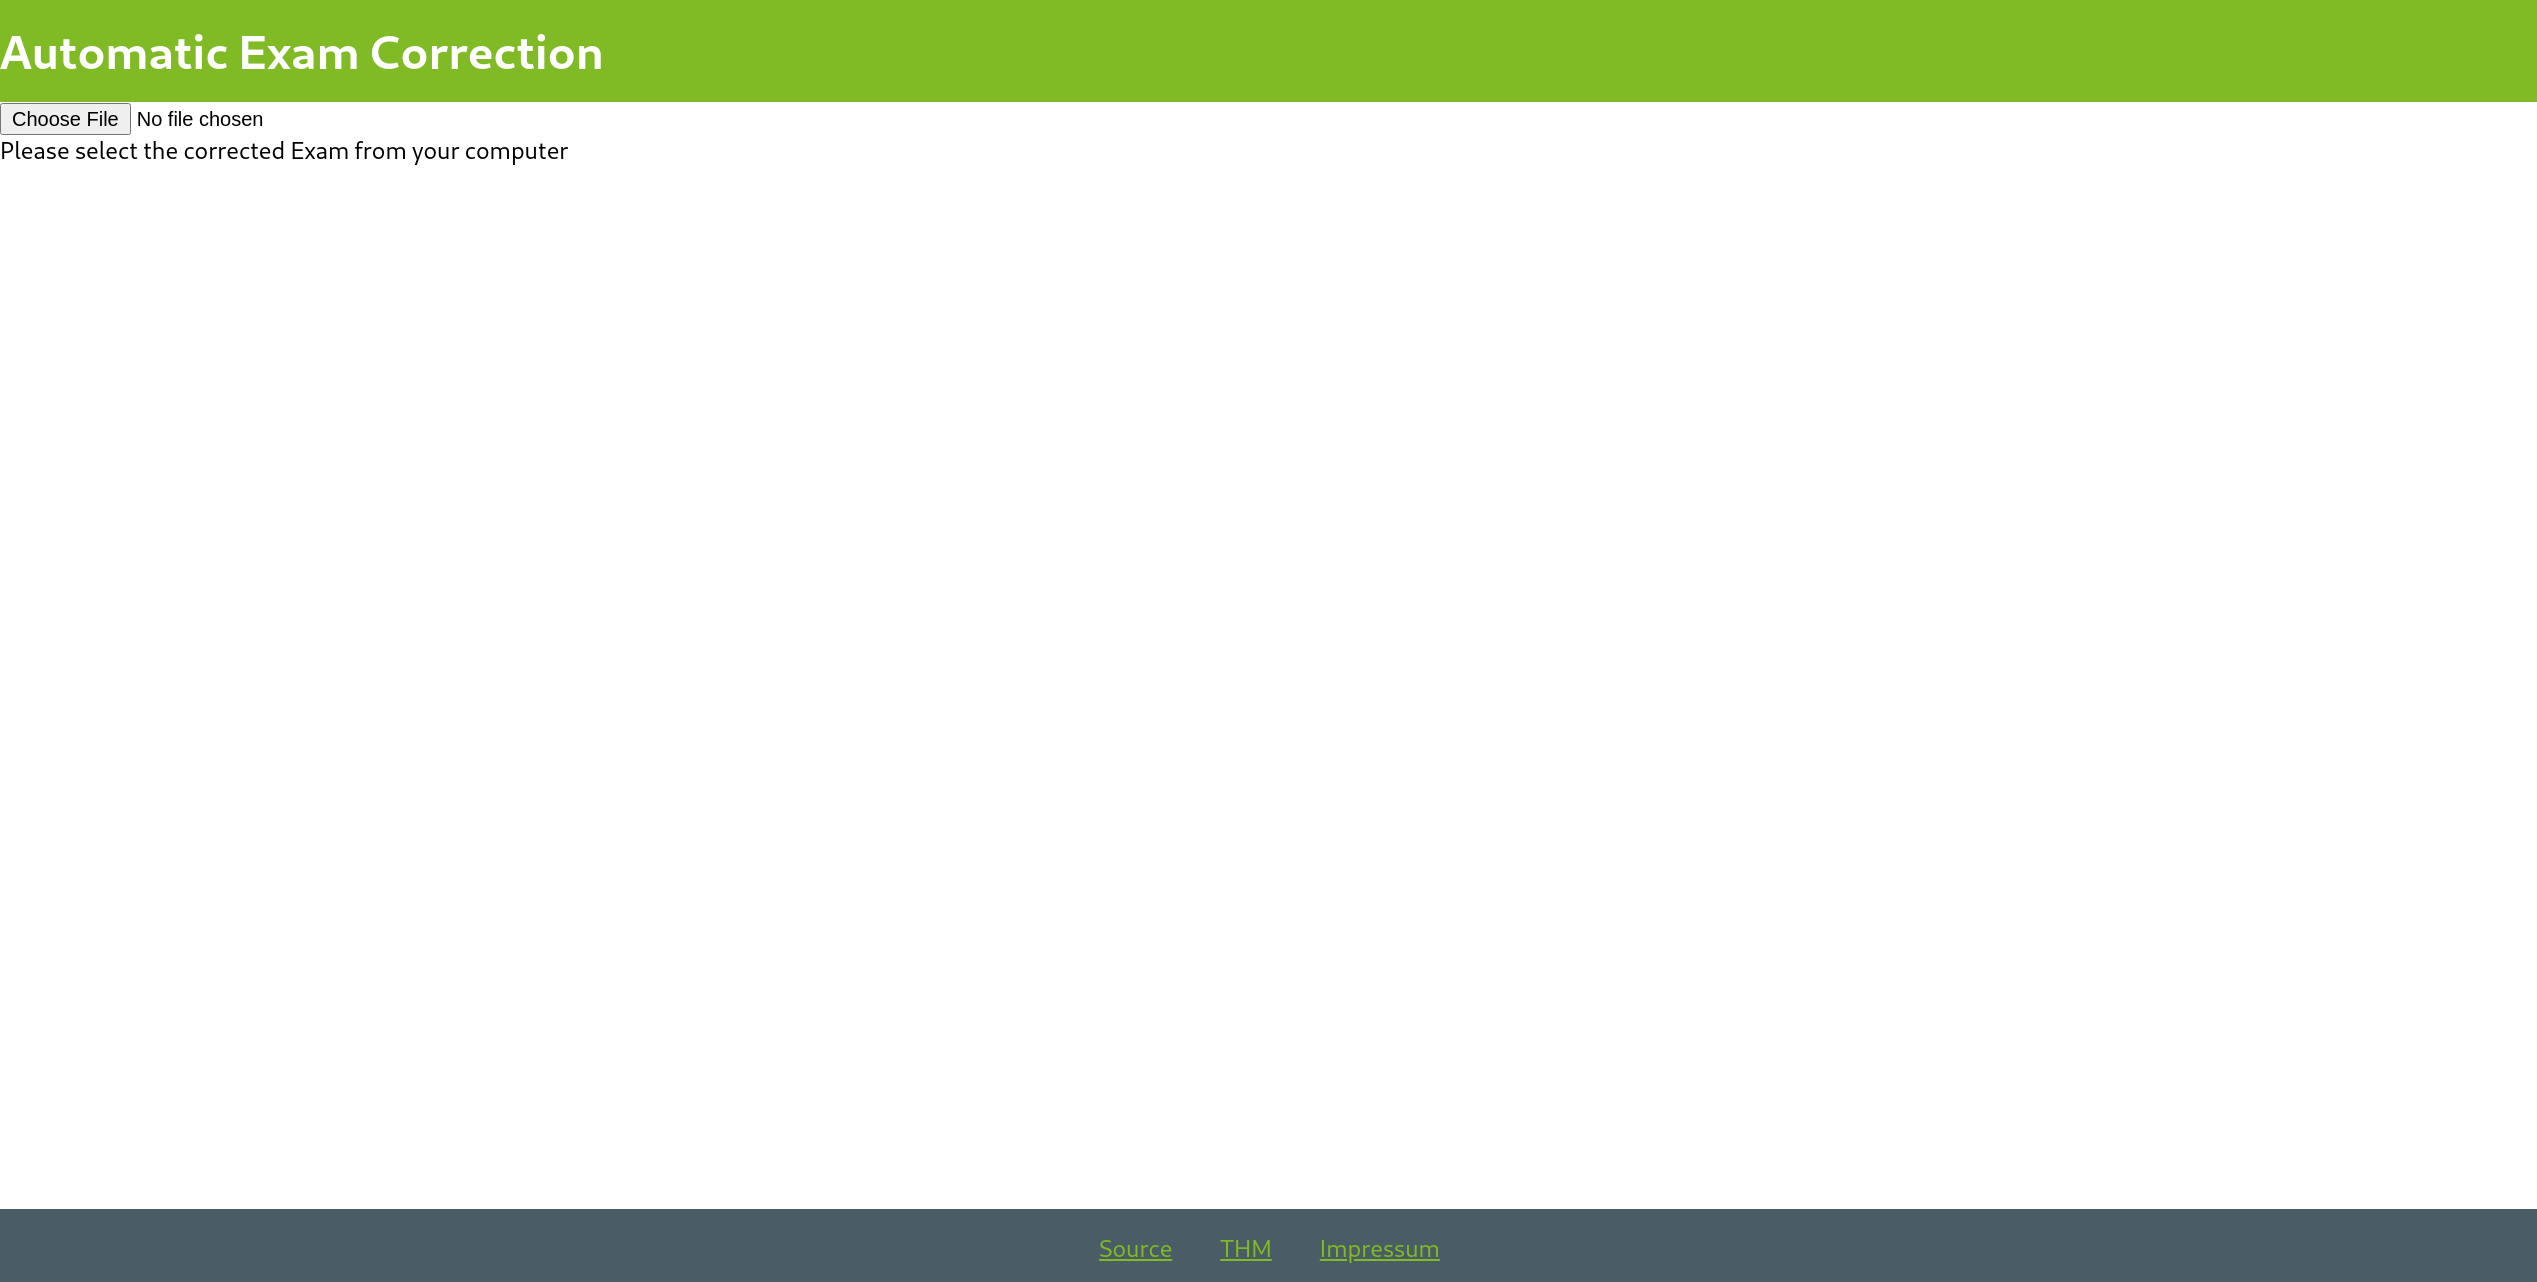
\includegraphics[width=\textwidth]{frontpage-view}
    \caption{Startseite der Automatic Exam Correction}
\end{figure}

\"Uber den Button oben links \texttt{Choose File} kann das erste Dokument geladen werden.
Hier ist zu beachten, dass dies ein entweder leeres Dokument oder eine korrekt ausgef\"ullte Mussterl\"osung sein sollte.

\subsection{Aufgaben Ausw\"ahlten}

Sobald dieses Dokument geladen ist, wird folgende Seite angezeigt.
Ab hier kann begonnen werden Aufgaben auszuw\"ahlen.

\begin{figure}[H]
\centering
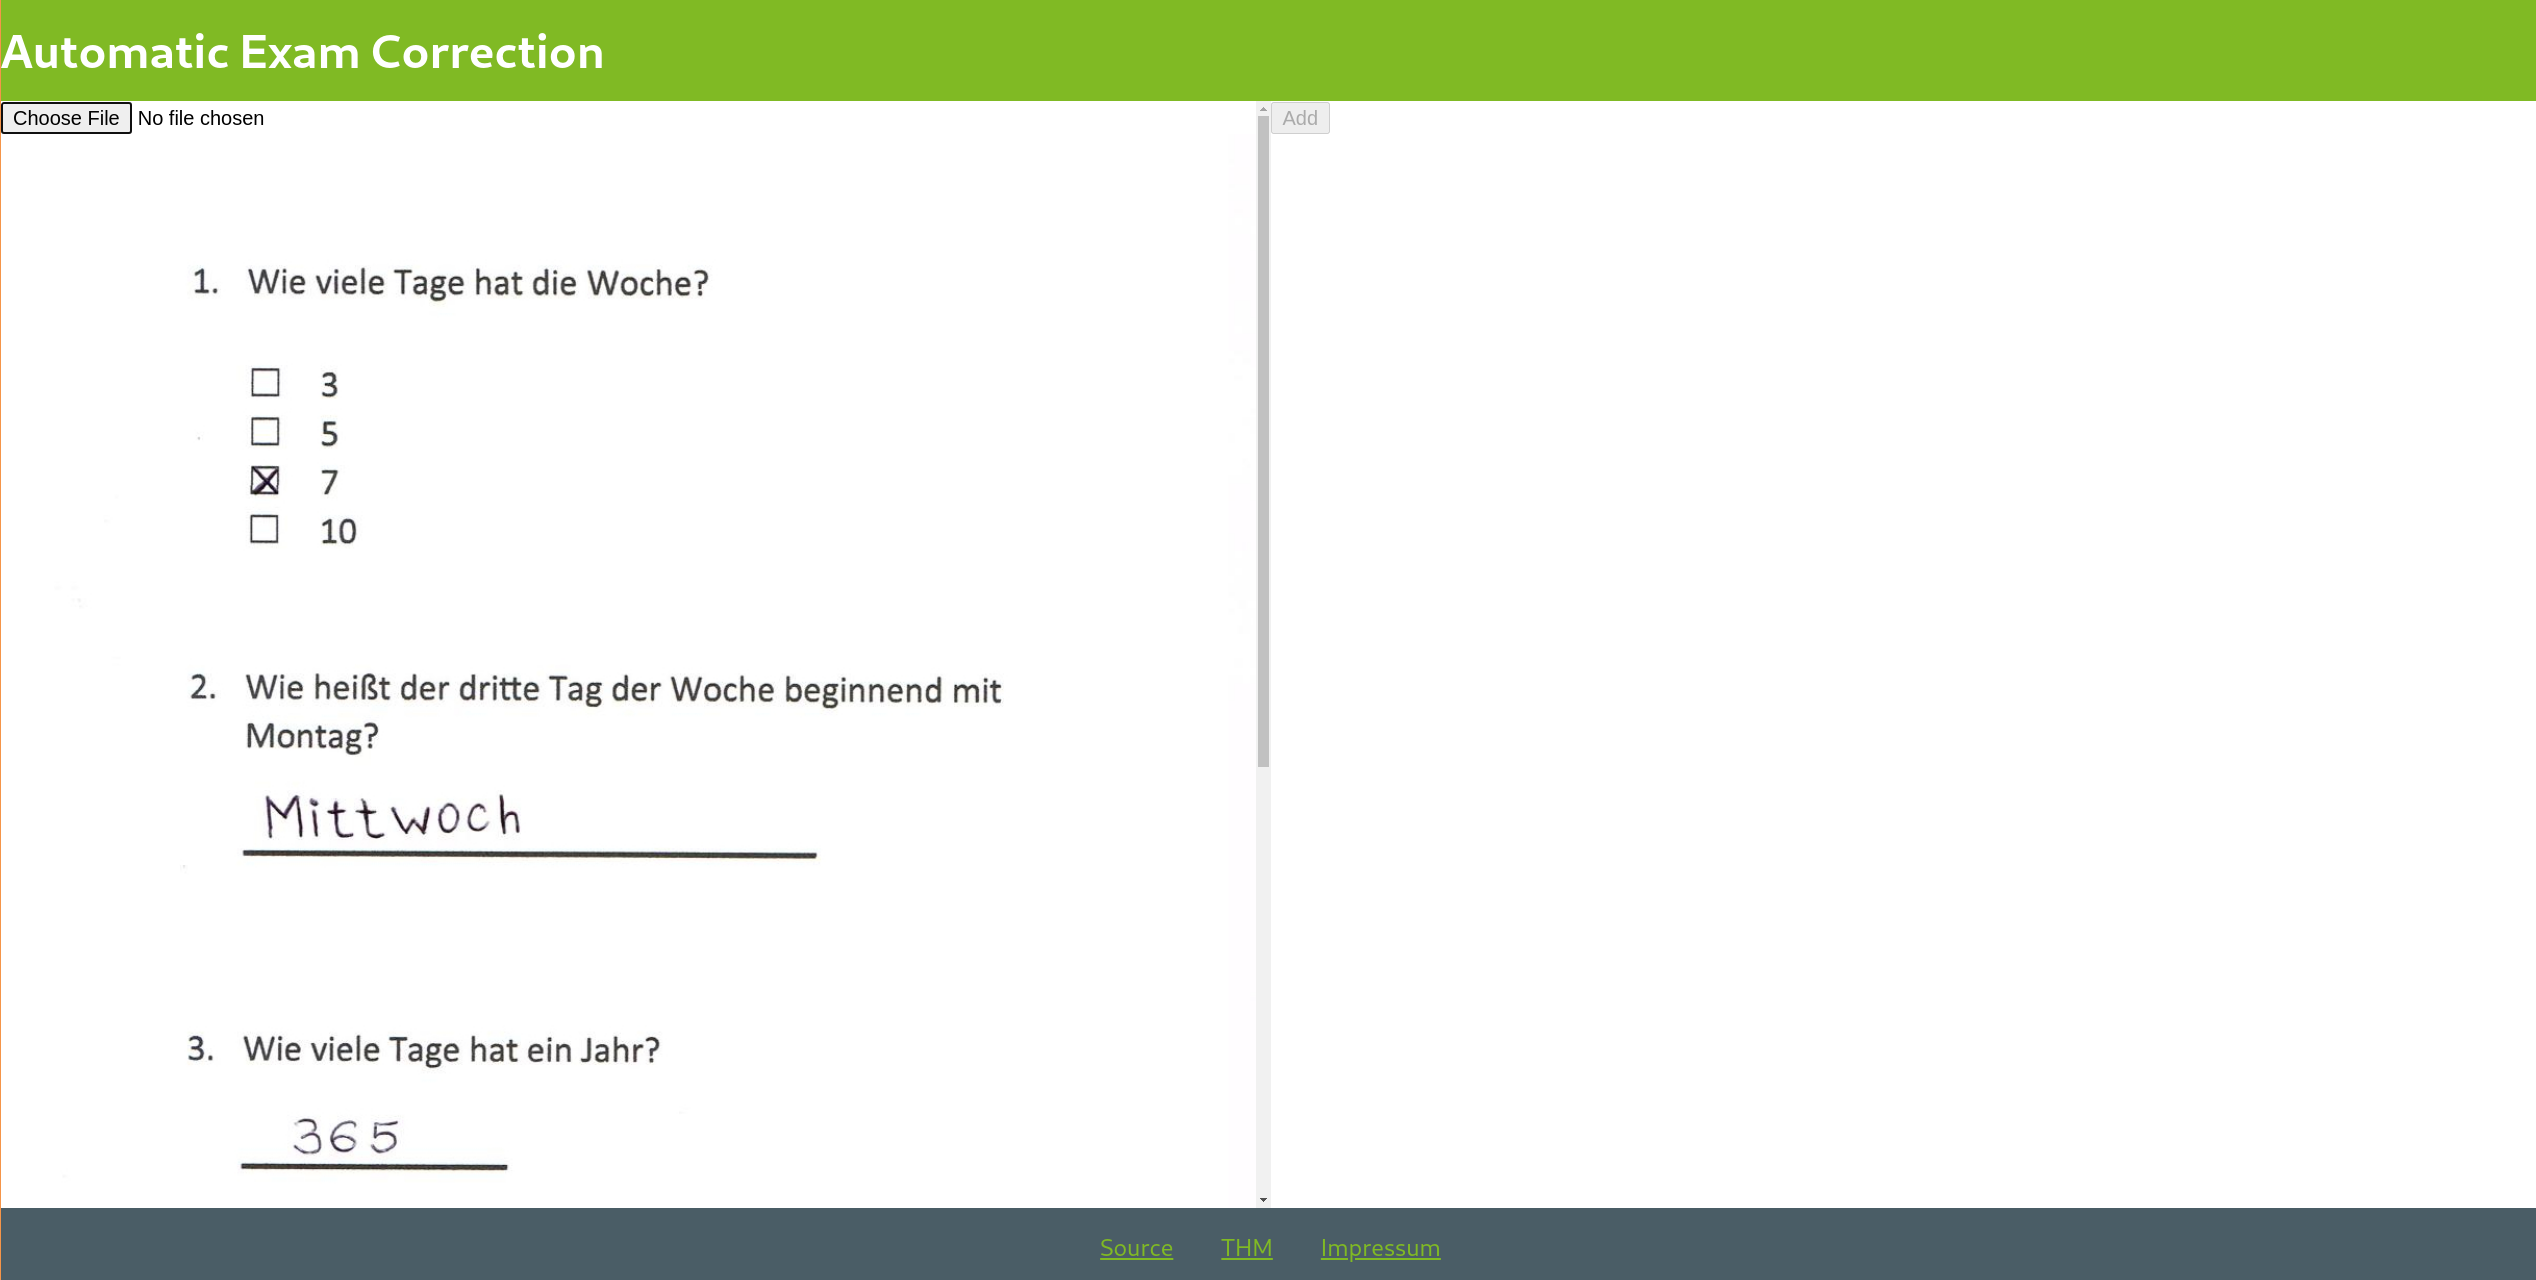
\includegraphics[width=\textwidth]{loaded-muster}
    \caption{Erstes geladene Dokument}
\end{figure}

Per Maus wird ein Bereich ausgew\"ahlt.
Dabei ist zu beachten, dass etwas Platz zwischen dem markierten Teil der Aufgabe und dem umliegendem Bereich gelassen wird.
Wichtig ist es nur den Teil zu markieren in dem auch eine Antwort erwartet wird, also nicht die Frage an sich zu markieren.

Mehr Informationen zu dem Thema "gut markieren" finden Sie in dem Kapitel "Aufgabentypen".

\begin{figure}[H]
\centering
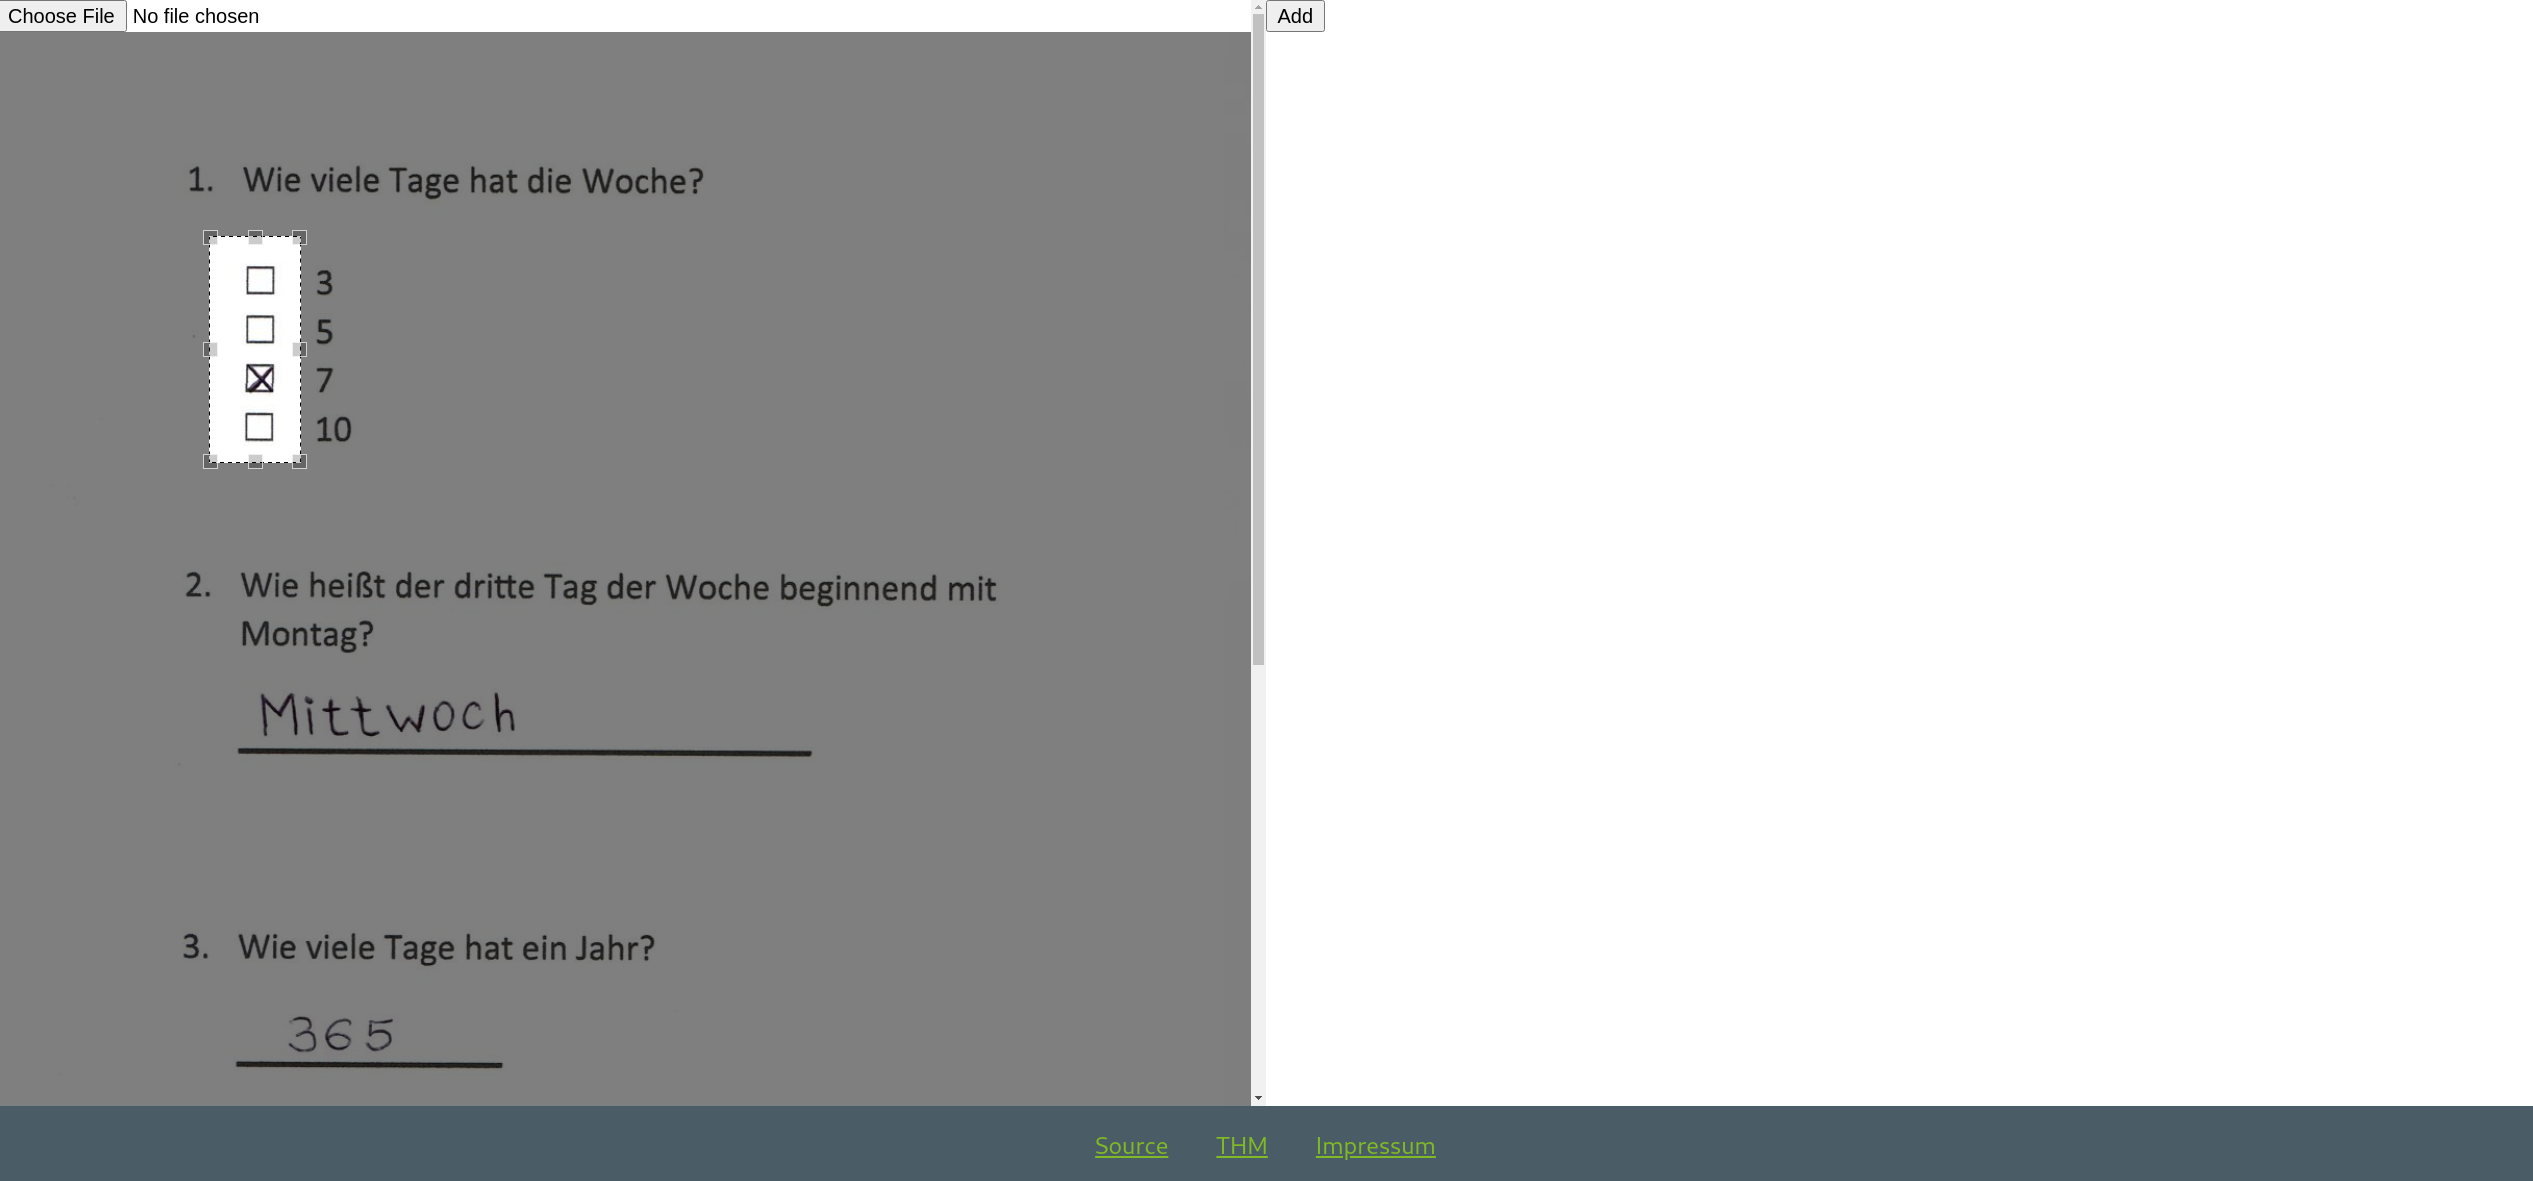
\includegraphics[width=\textwidth]{select-task}
    \caption{Beispiel zum ausgewählten Aufgabenbereich}
\end{figure}

Wenn auf den \texttt{Add} Butten geklickt wurde, erscheint folgende Darstellung:

\begin{figure}[H]
\centering
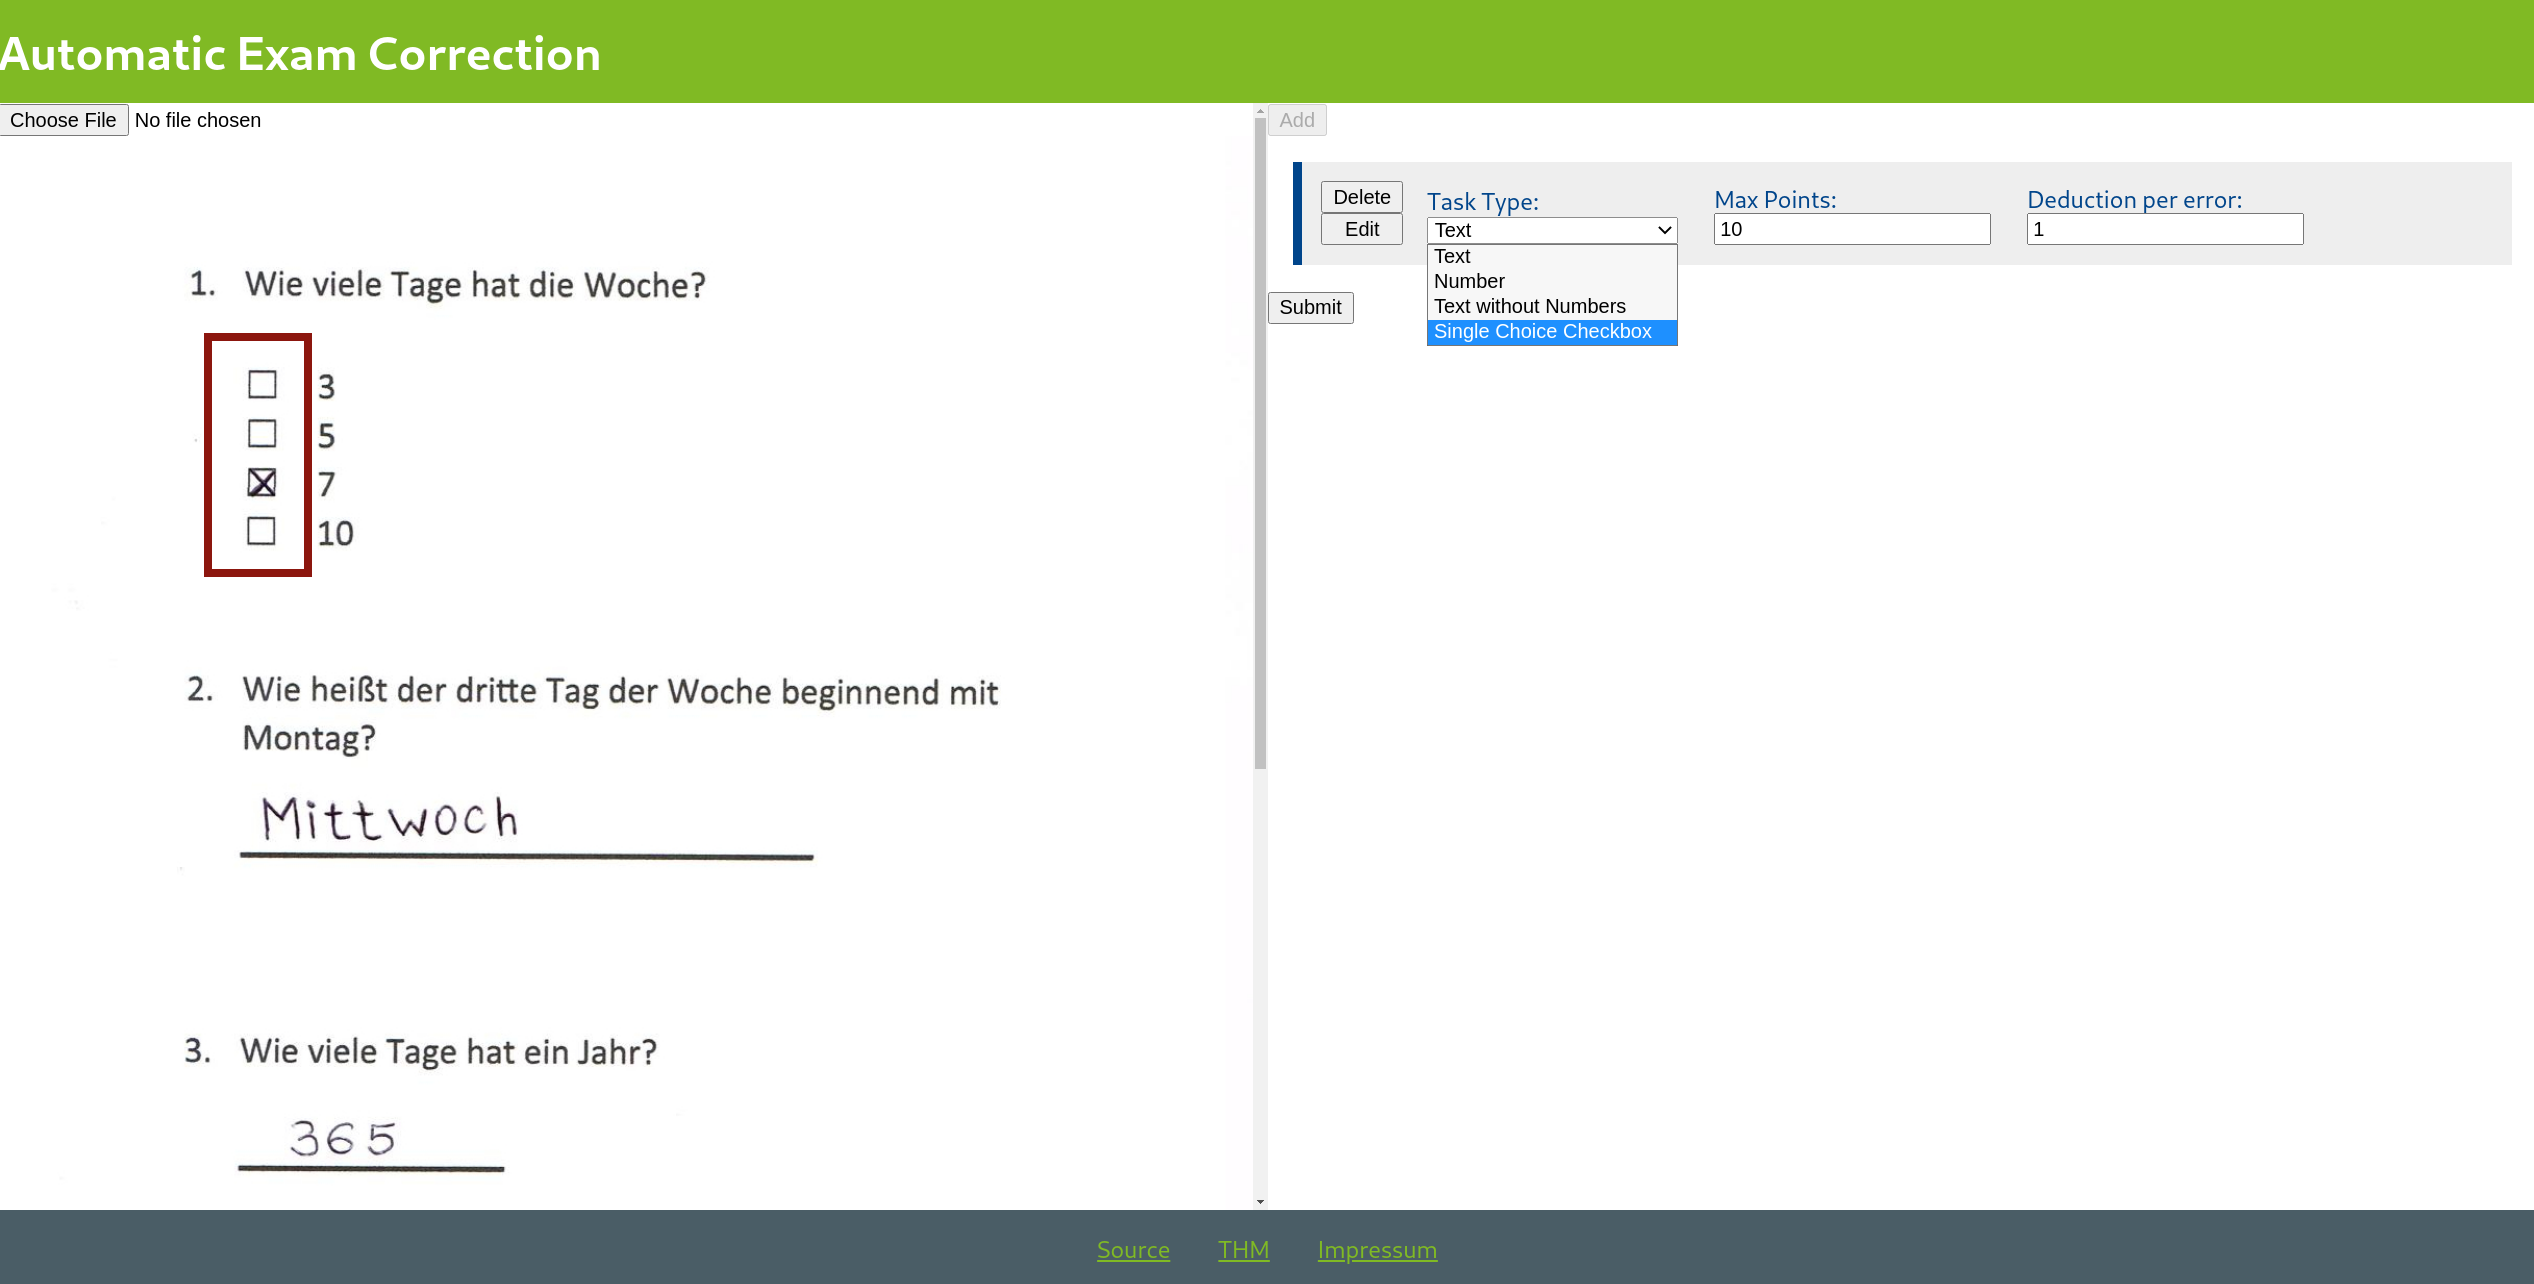
\includegraphics[width=\textwidth]{select-task-type}
    \caption{Auswahl des Aufgaben Typs}
\end{figure}

Hier kann der Aufgabentyp, die maximalen Punkte und der Abzug pro Fehler gesetzt werden.
So kann mit dem Button \texttt{Delete} auch die Auswahl gel\"oscht werden und mit dem Button \texttt{Edit} der ausgew\"ahlte Bereich ver\"andert werden.

Im folgendem Bild sind nun mehrere Aufgaben ausgew\"ahlt:

\begin{figure}[H]
\centering
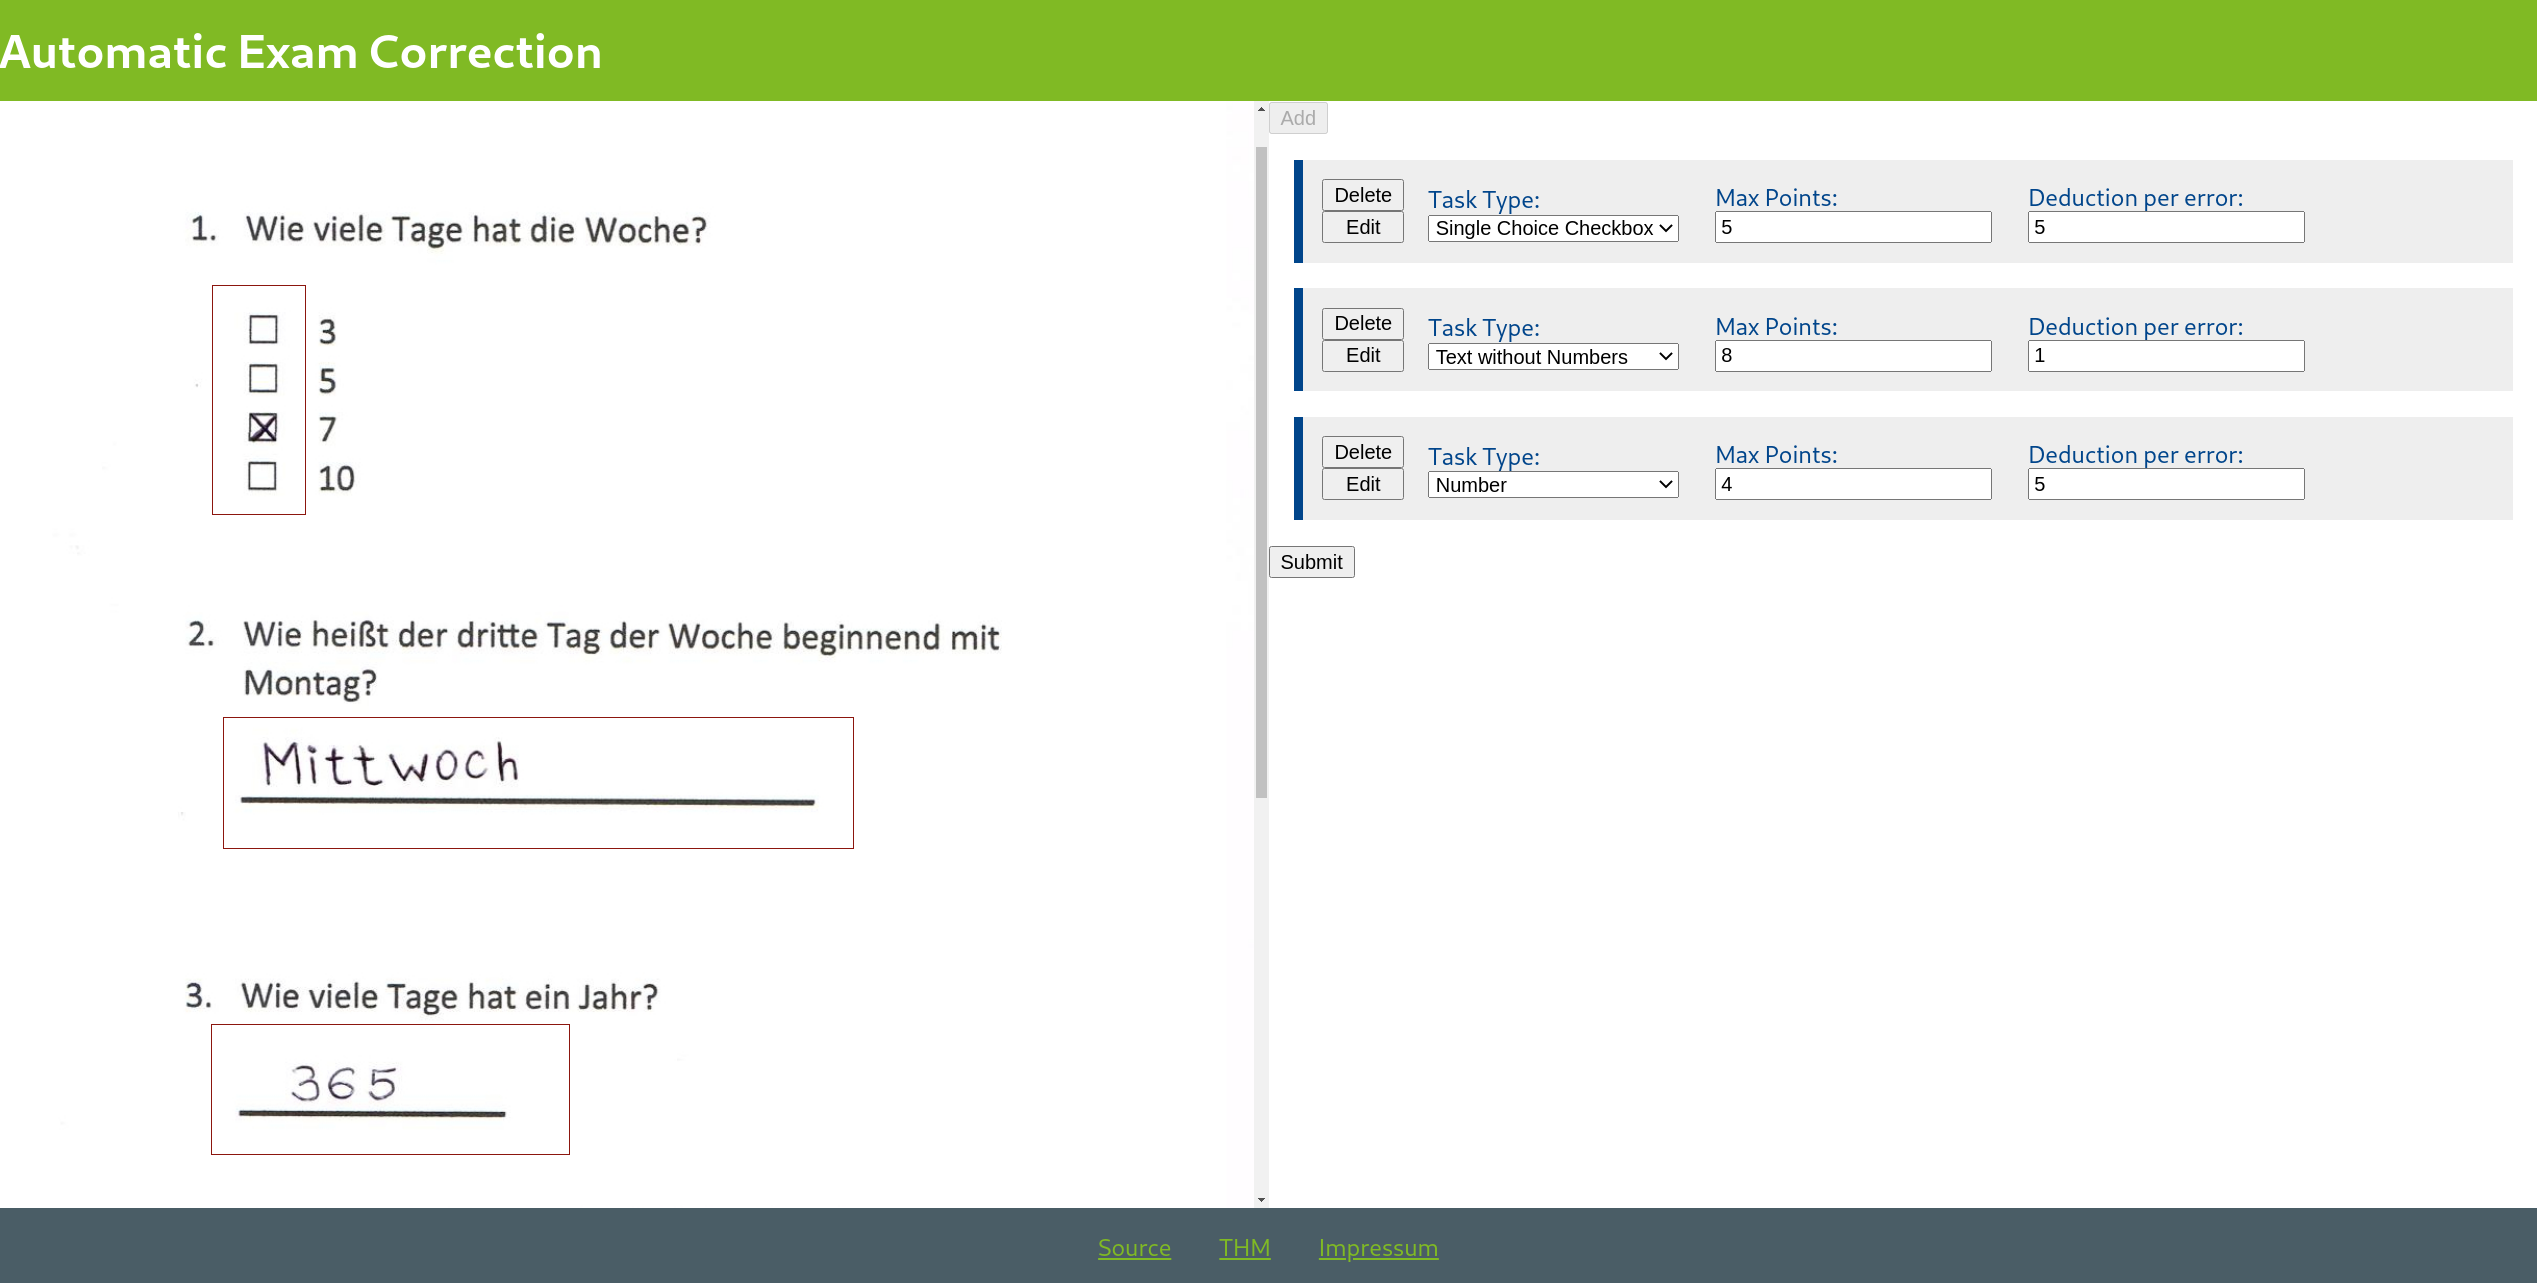
\includegraphics[width=\textwidth]{multiple-tasks-set-points}
    \caption{Auswahl mehrerer Aufgaben}
\end{figure}
Es ist hier besonders zu beachten die Aufgabentypen \texttt{text}, \texttt{numbers} und \texttt{text without numbers} entsprechend zu setzen.
Dies erh\"ot die Genauigkeit der automatischen Erkennung.
Wenn alles nun noch einmal kontrolliert wurde, kann der "Submit" Button gedr\"uckt werden.
Dadurch werden die ausgew\"ahlten Bereiche automatisch verarbeitet.

\subsection{Erkennung von Musterl\"osung und Laden der Formulare}

Es ist wichtig, dass die erkannten Aufgaben von einem Menschen noch einmal durchgesehen werden, weil die automatische Erkennung nicht immer korrekt ist.
Dazu kann man in der n\"achsten Ansicht einfach auf die Textfelder die mit "Correct Answer" beschrieben sind klicken und dort den korrekten Text eingeben.

\begin{figure}[H]
\centering
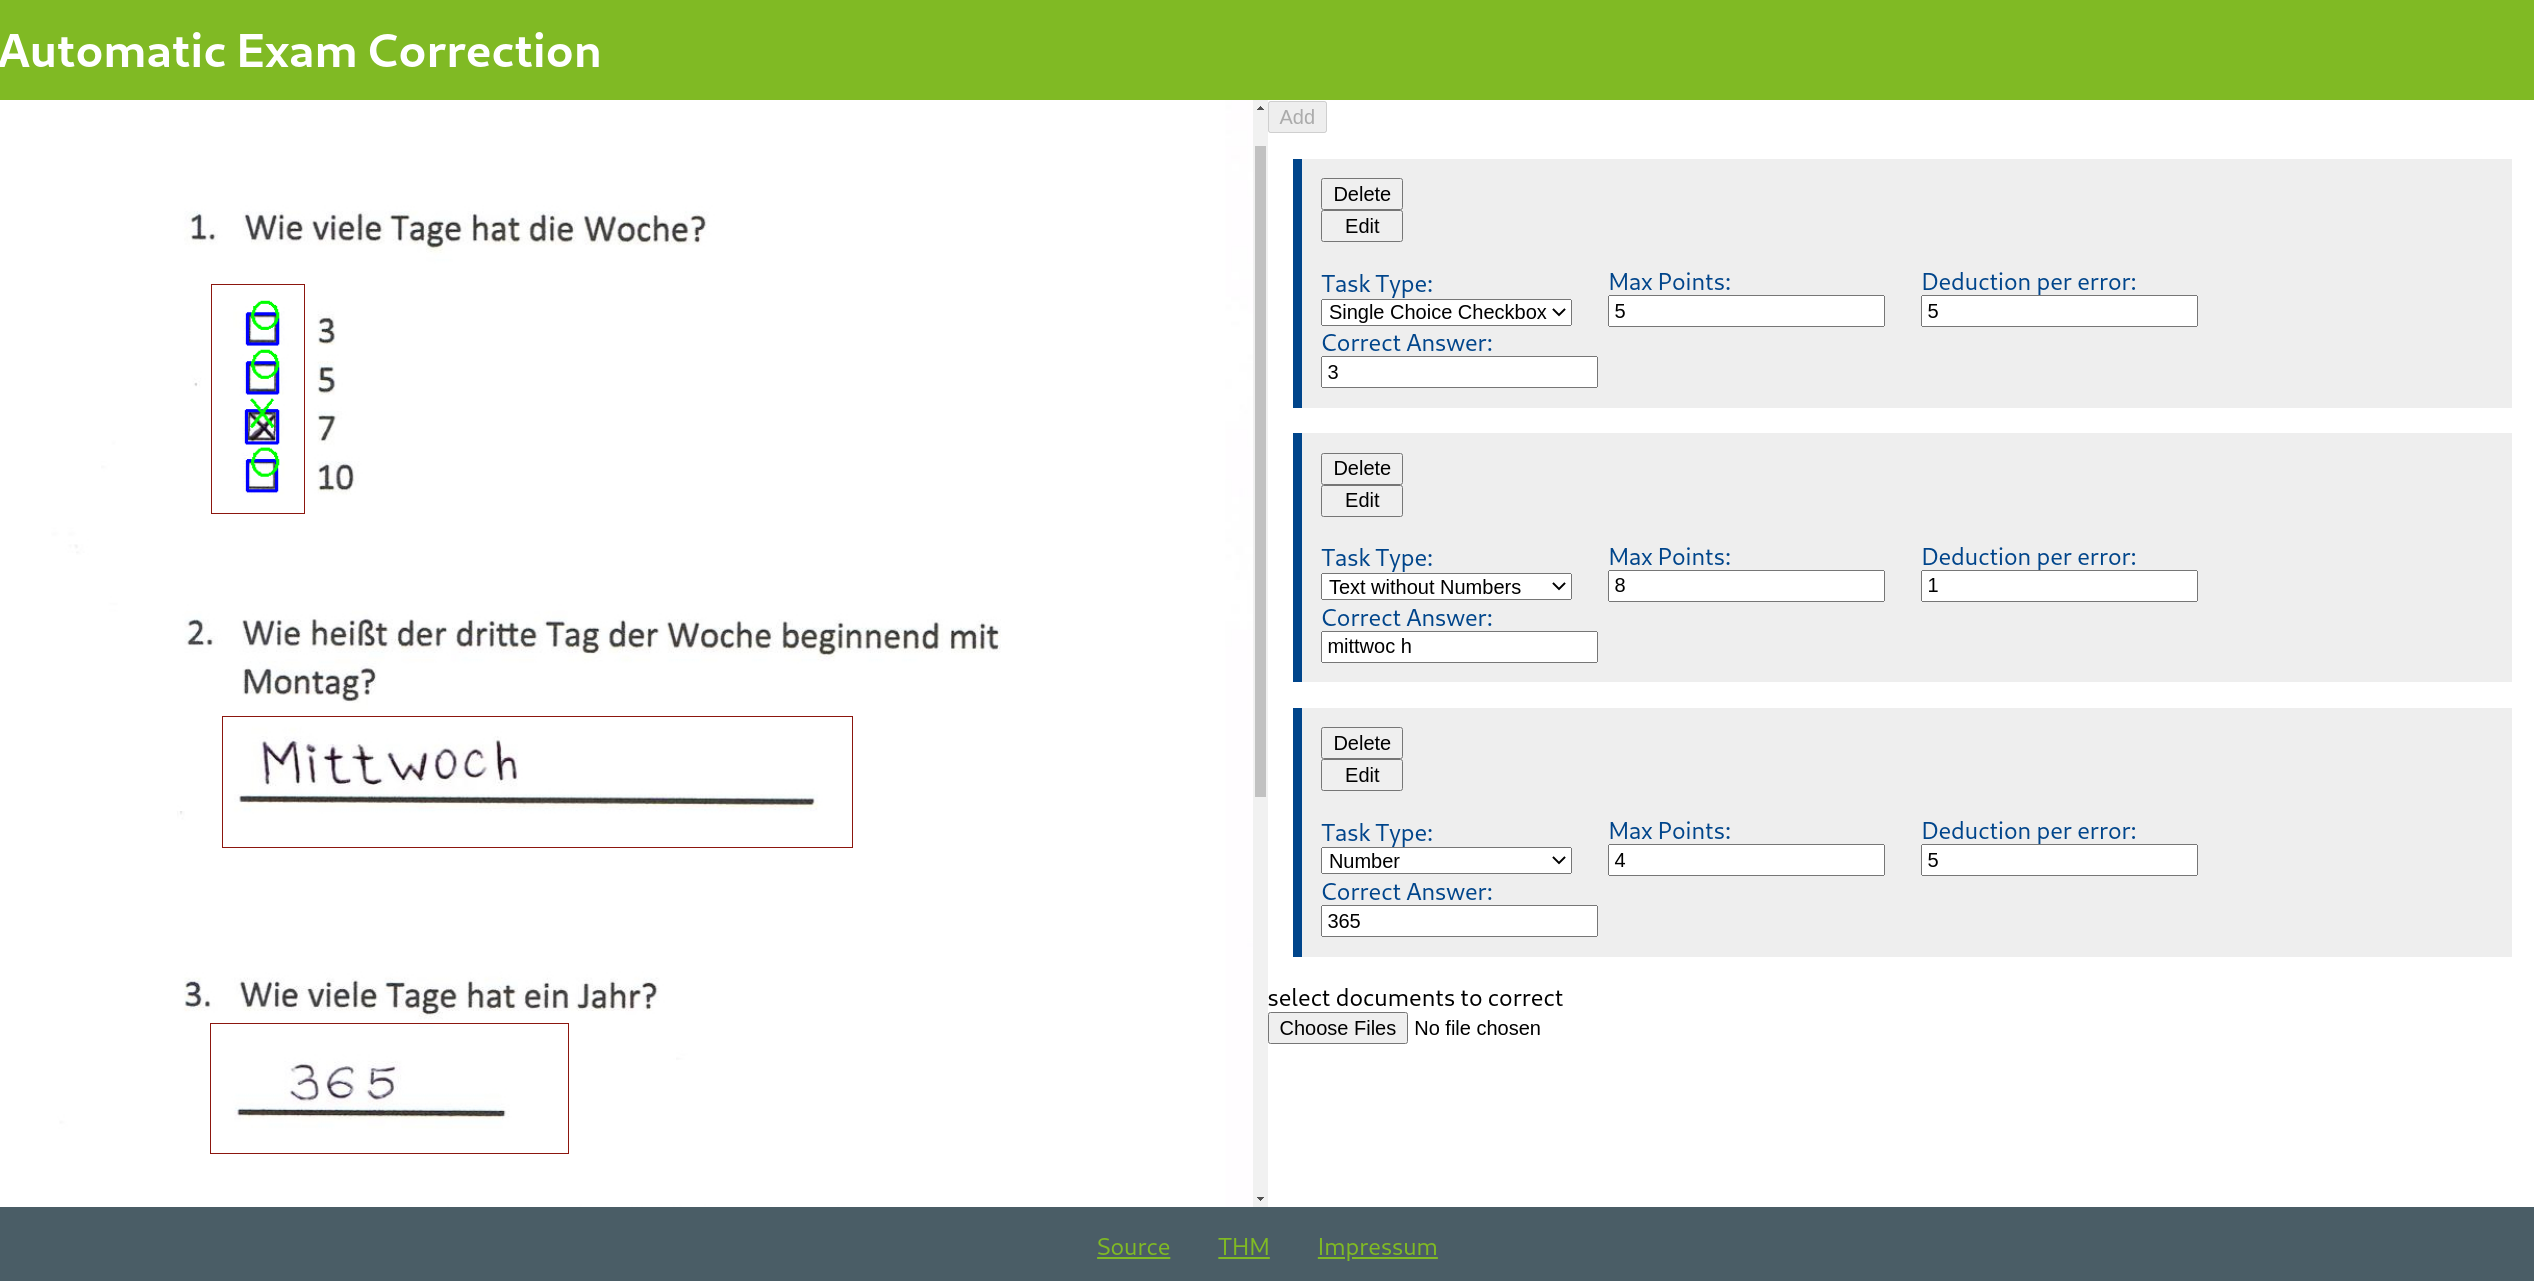
\includegraphics[width=\textwidth]{detected-sample-solition}
    \caption{Möglichkeit zur Nachbesserung}
\end{figure}

Darauf sollten dann die korrekten Antworten gesetzt und die gew\"unschten Punktzahlen eingetragen sein.

\begin{figure}[H]
\centering
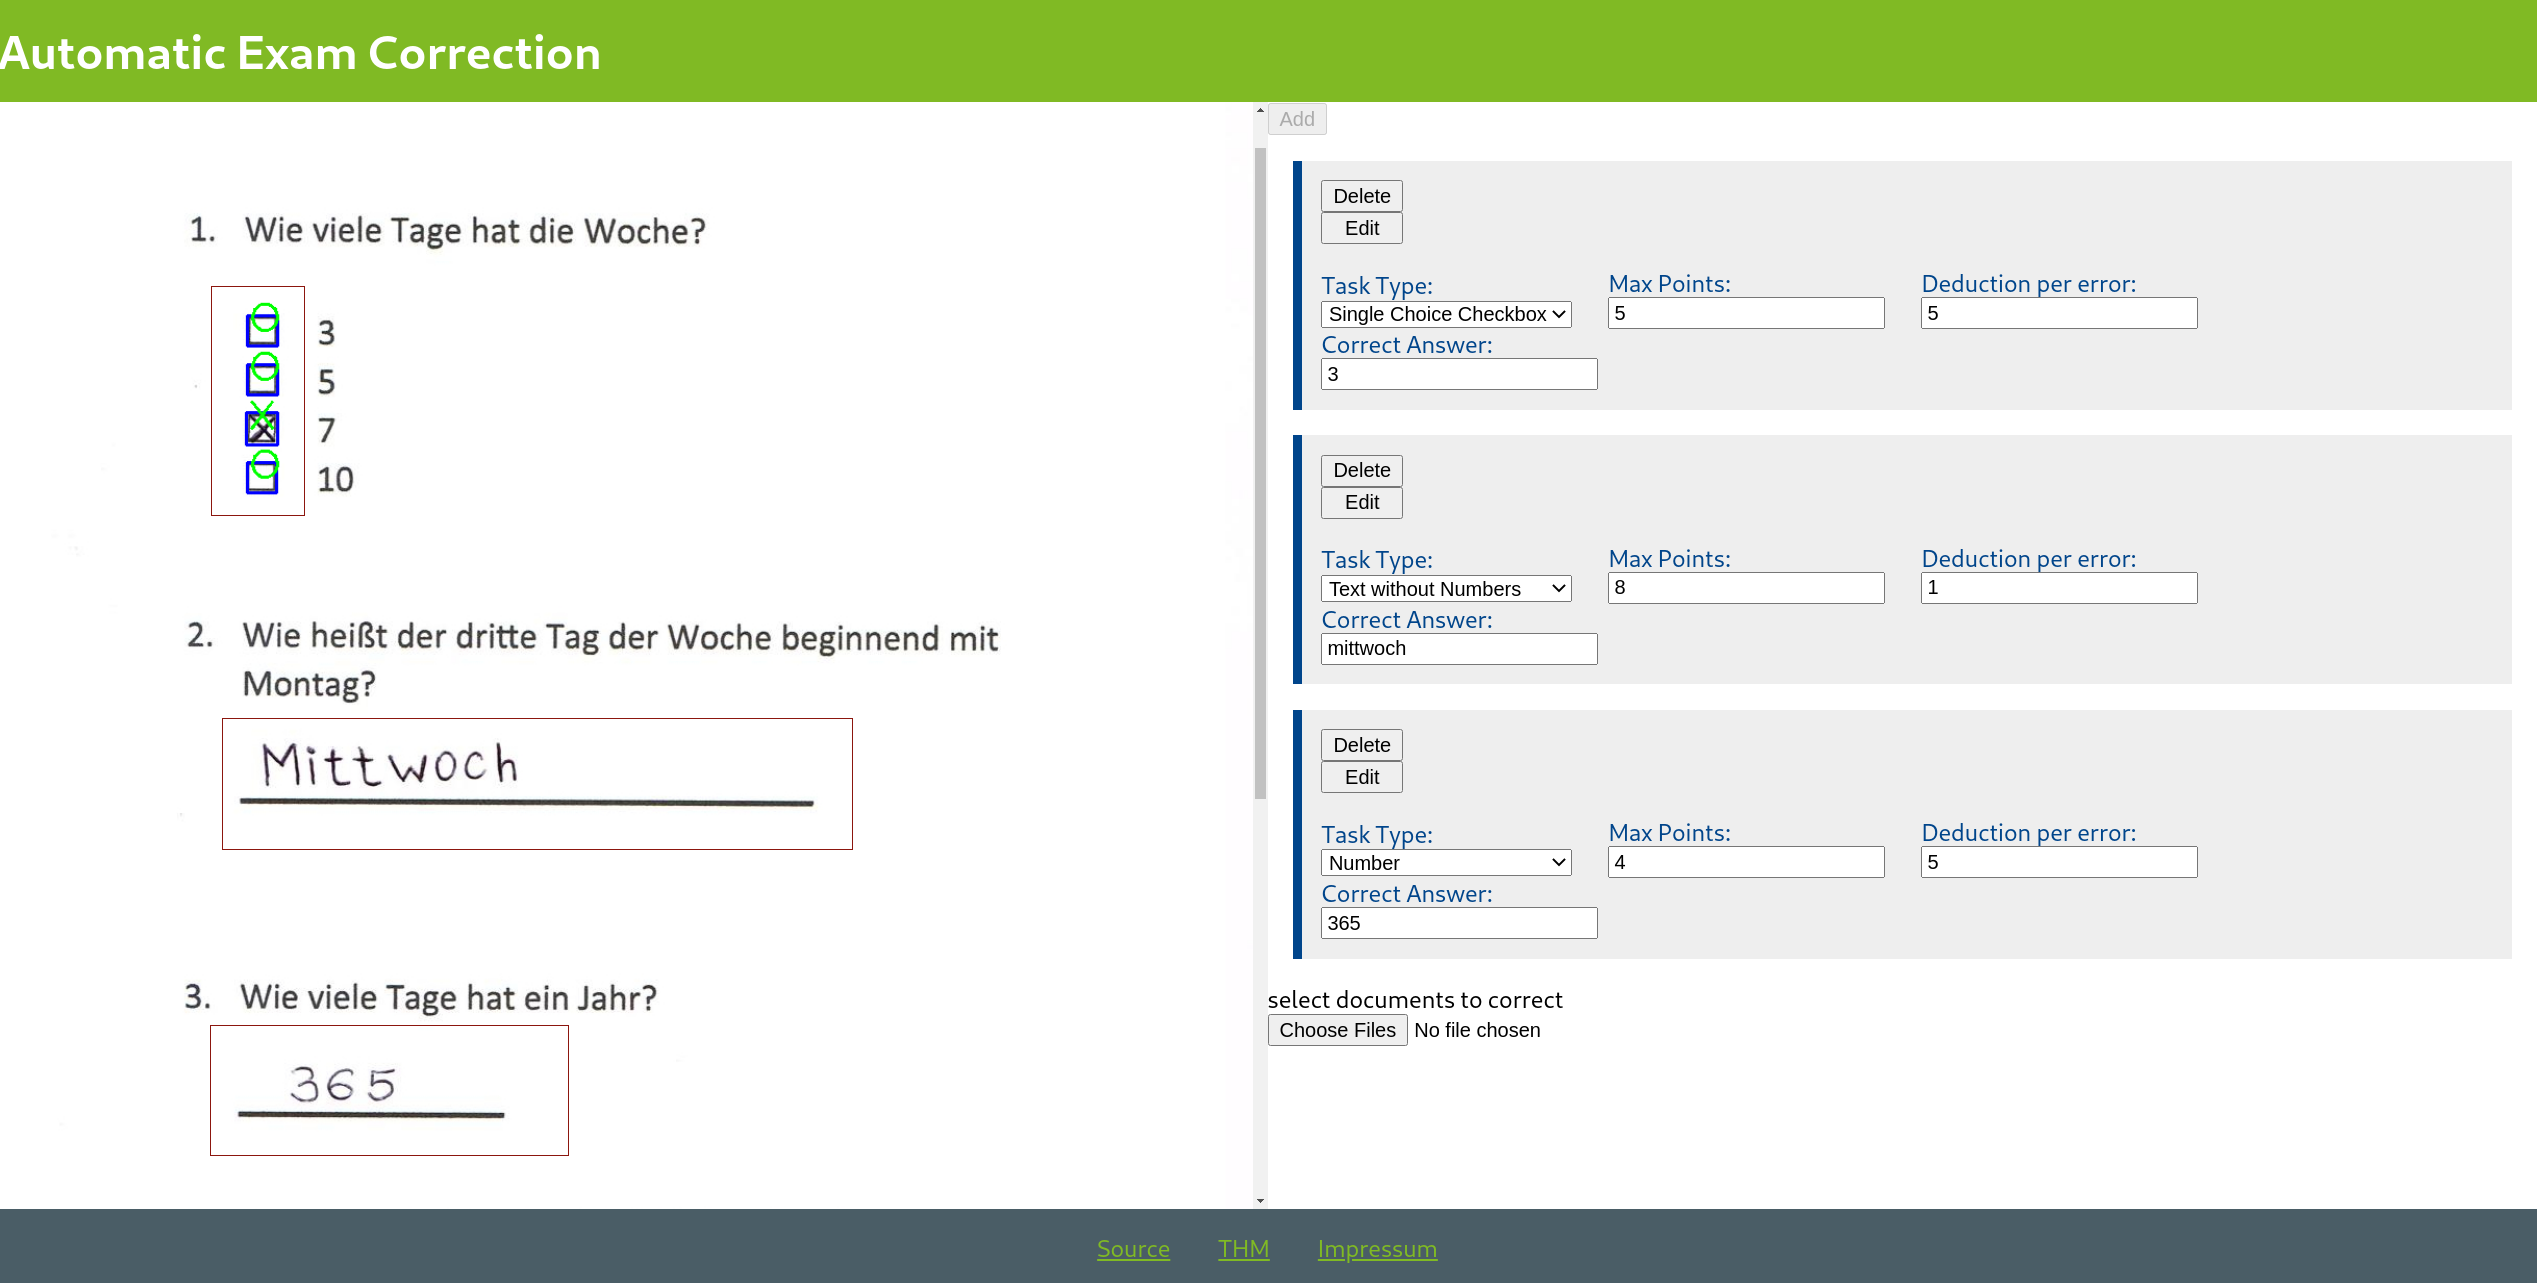
\includegraphics[width=\textwidth]{detected-sample-solition-corrected}
    \caption{Nachgebesserte Fassung}
\end{figure}

Nun k\"onnen mit dem Button \texttt{Choose Files} ein oder mehrere zu korrigierende Formulare ausgew\"ahlt werden.
Sobald dies geschehen ist, erscheint der \texttt{Next} Button.

\begin{figure}[H]
\centering
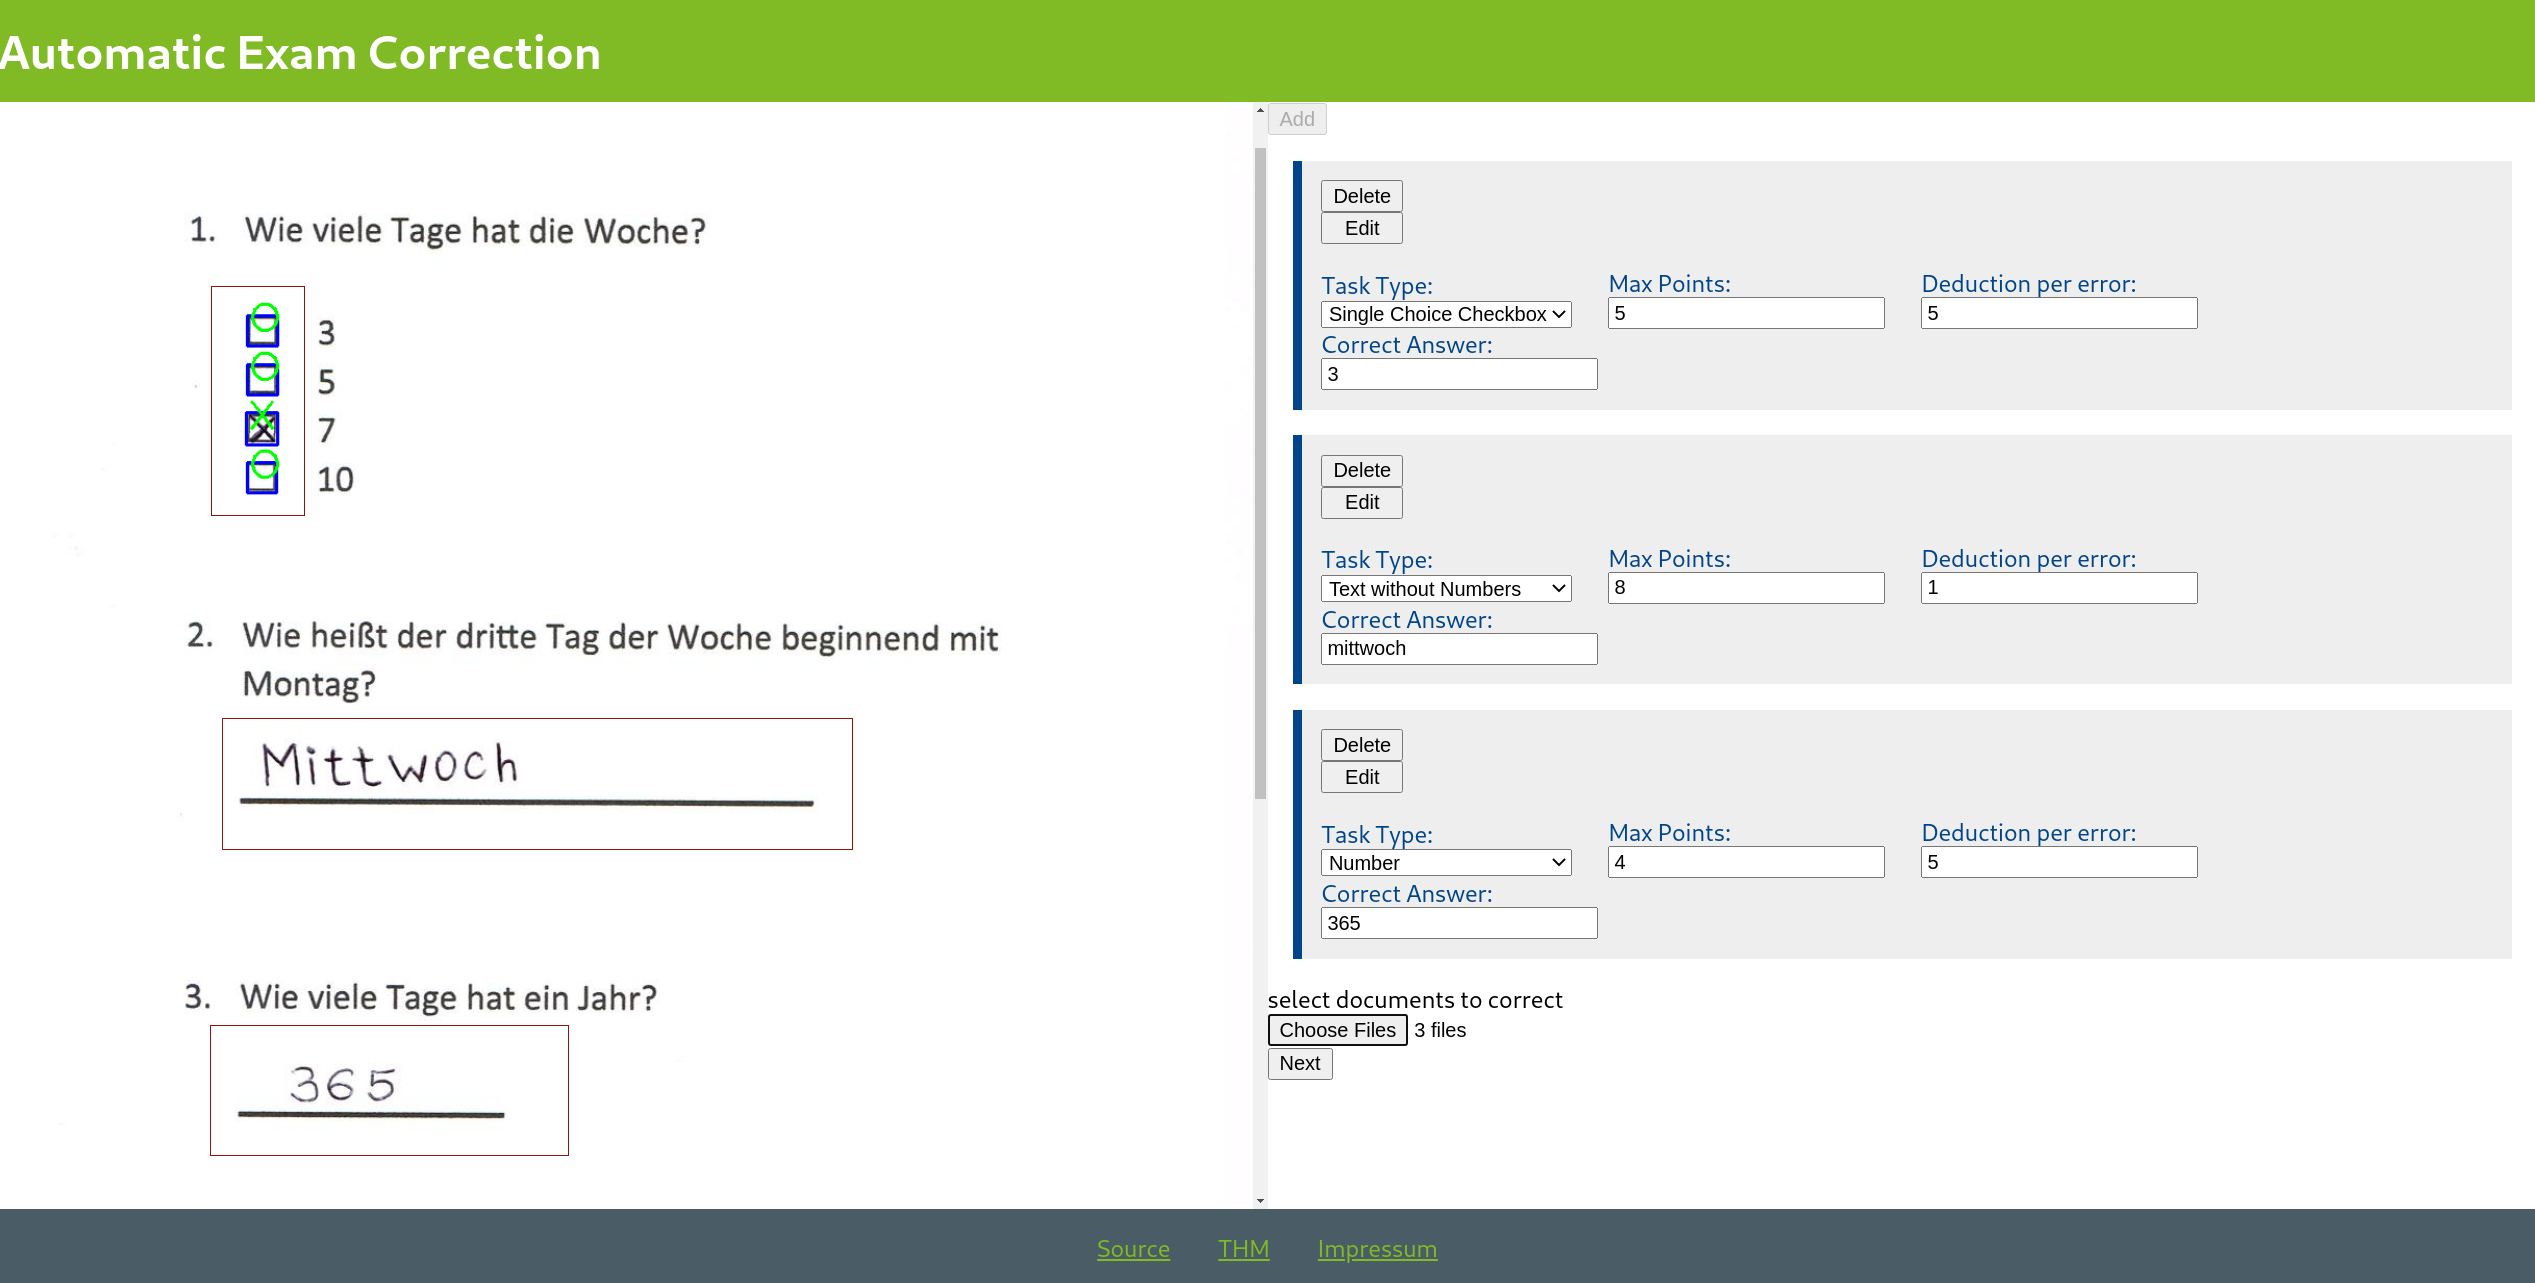
\includegraphics[width=\textwidth]{exams-selected}
    \caption{\texttt{Next} Button ist auf der rechten Seite erschienen}
\end{figure}

\subsection{Korrigierte Formulare \"Ubersicht und Korrektur}

Nun bekommt man eine \"Ubersicht aller korrigierten Formulare.
Rechts sind die Durchschnitte der einzelnen Aufgaben und links die einzelnen Formulare zu sehen.

\begin{figure}[H]
\centering
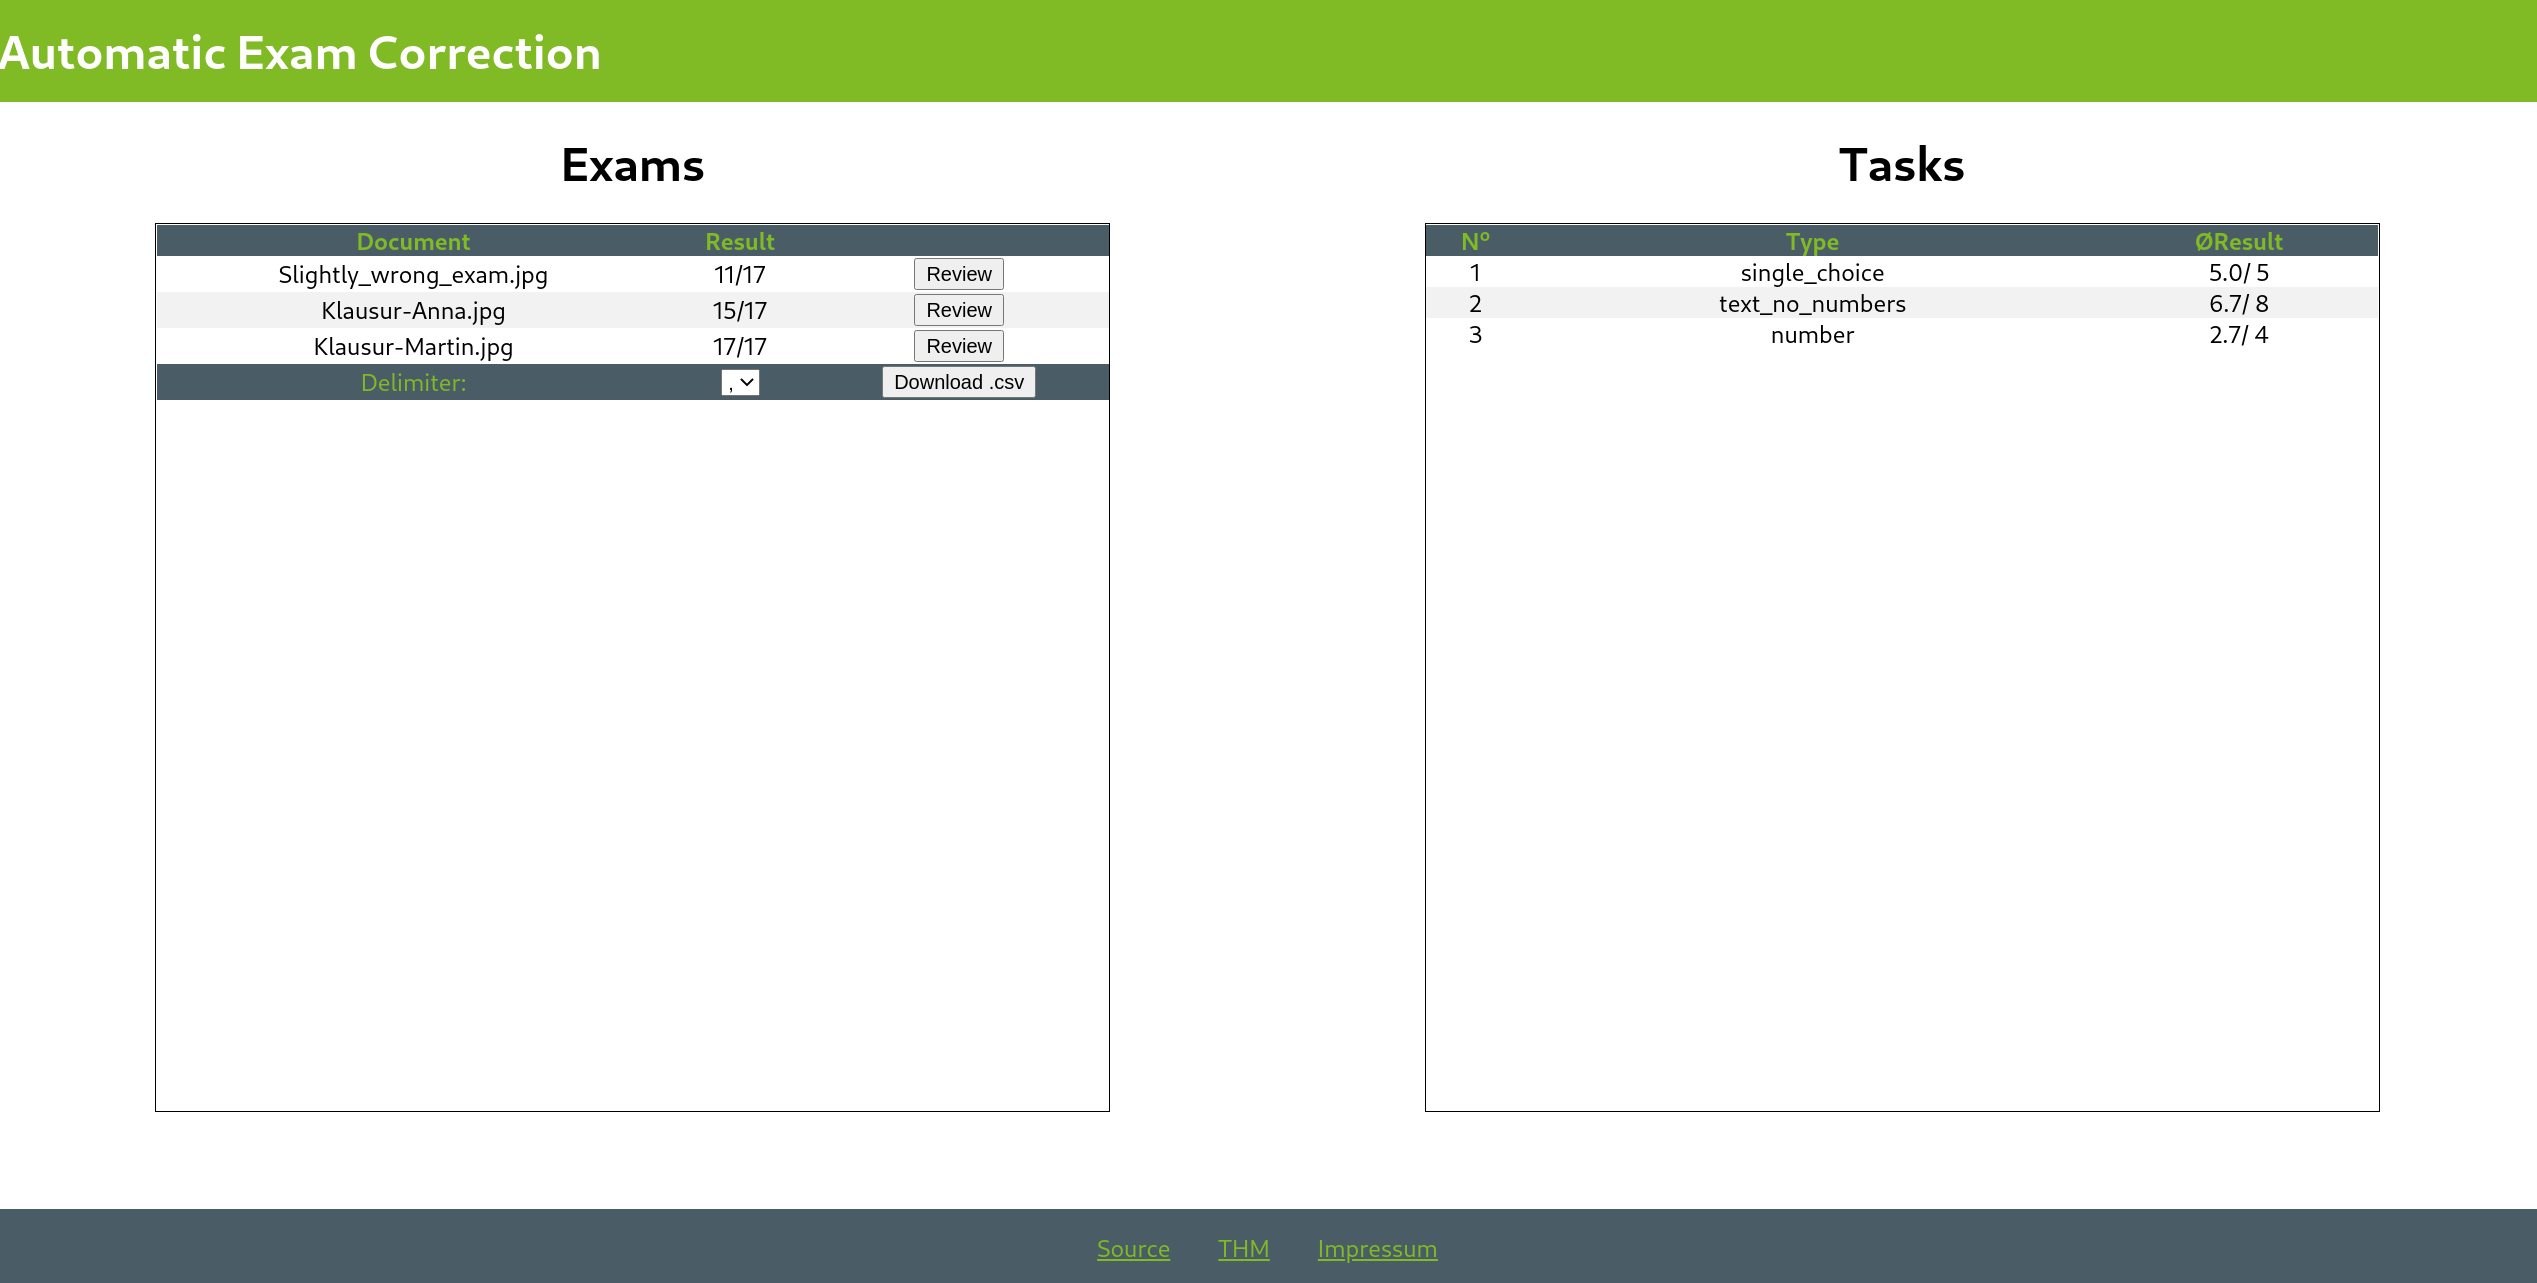
\includegraphics[width=\textwidth]{review-overview}
    \caption{Ansicht über die korrigierten Prüfungen}
\end{figure}

Wird auf der linken Seite bei einer der Formulare auf \texttt{Review} geklickt, \"offnet sich das Formular.
Dort kann gepr\"uft werden, ob die Aufgaben korrekt erkannt wurden.
Au{\ss}erdem k\"onnen hier die Punktzahlen der Aufgaben ver\"andert werden.

\begin{figure}[H]
\centering
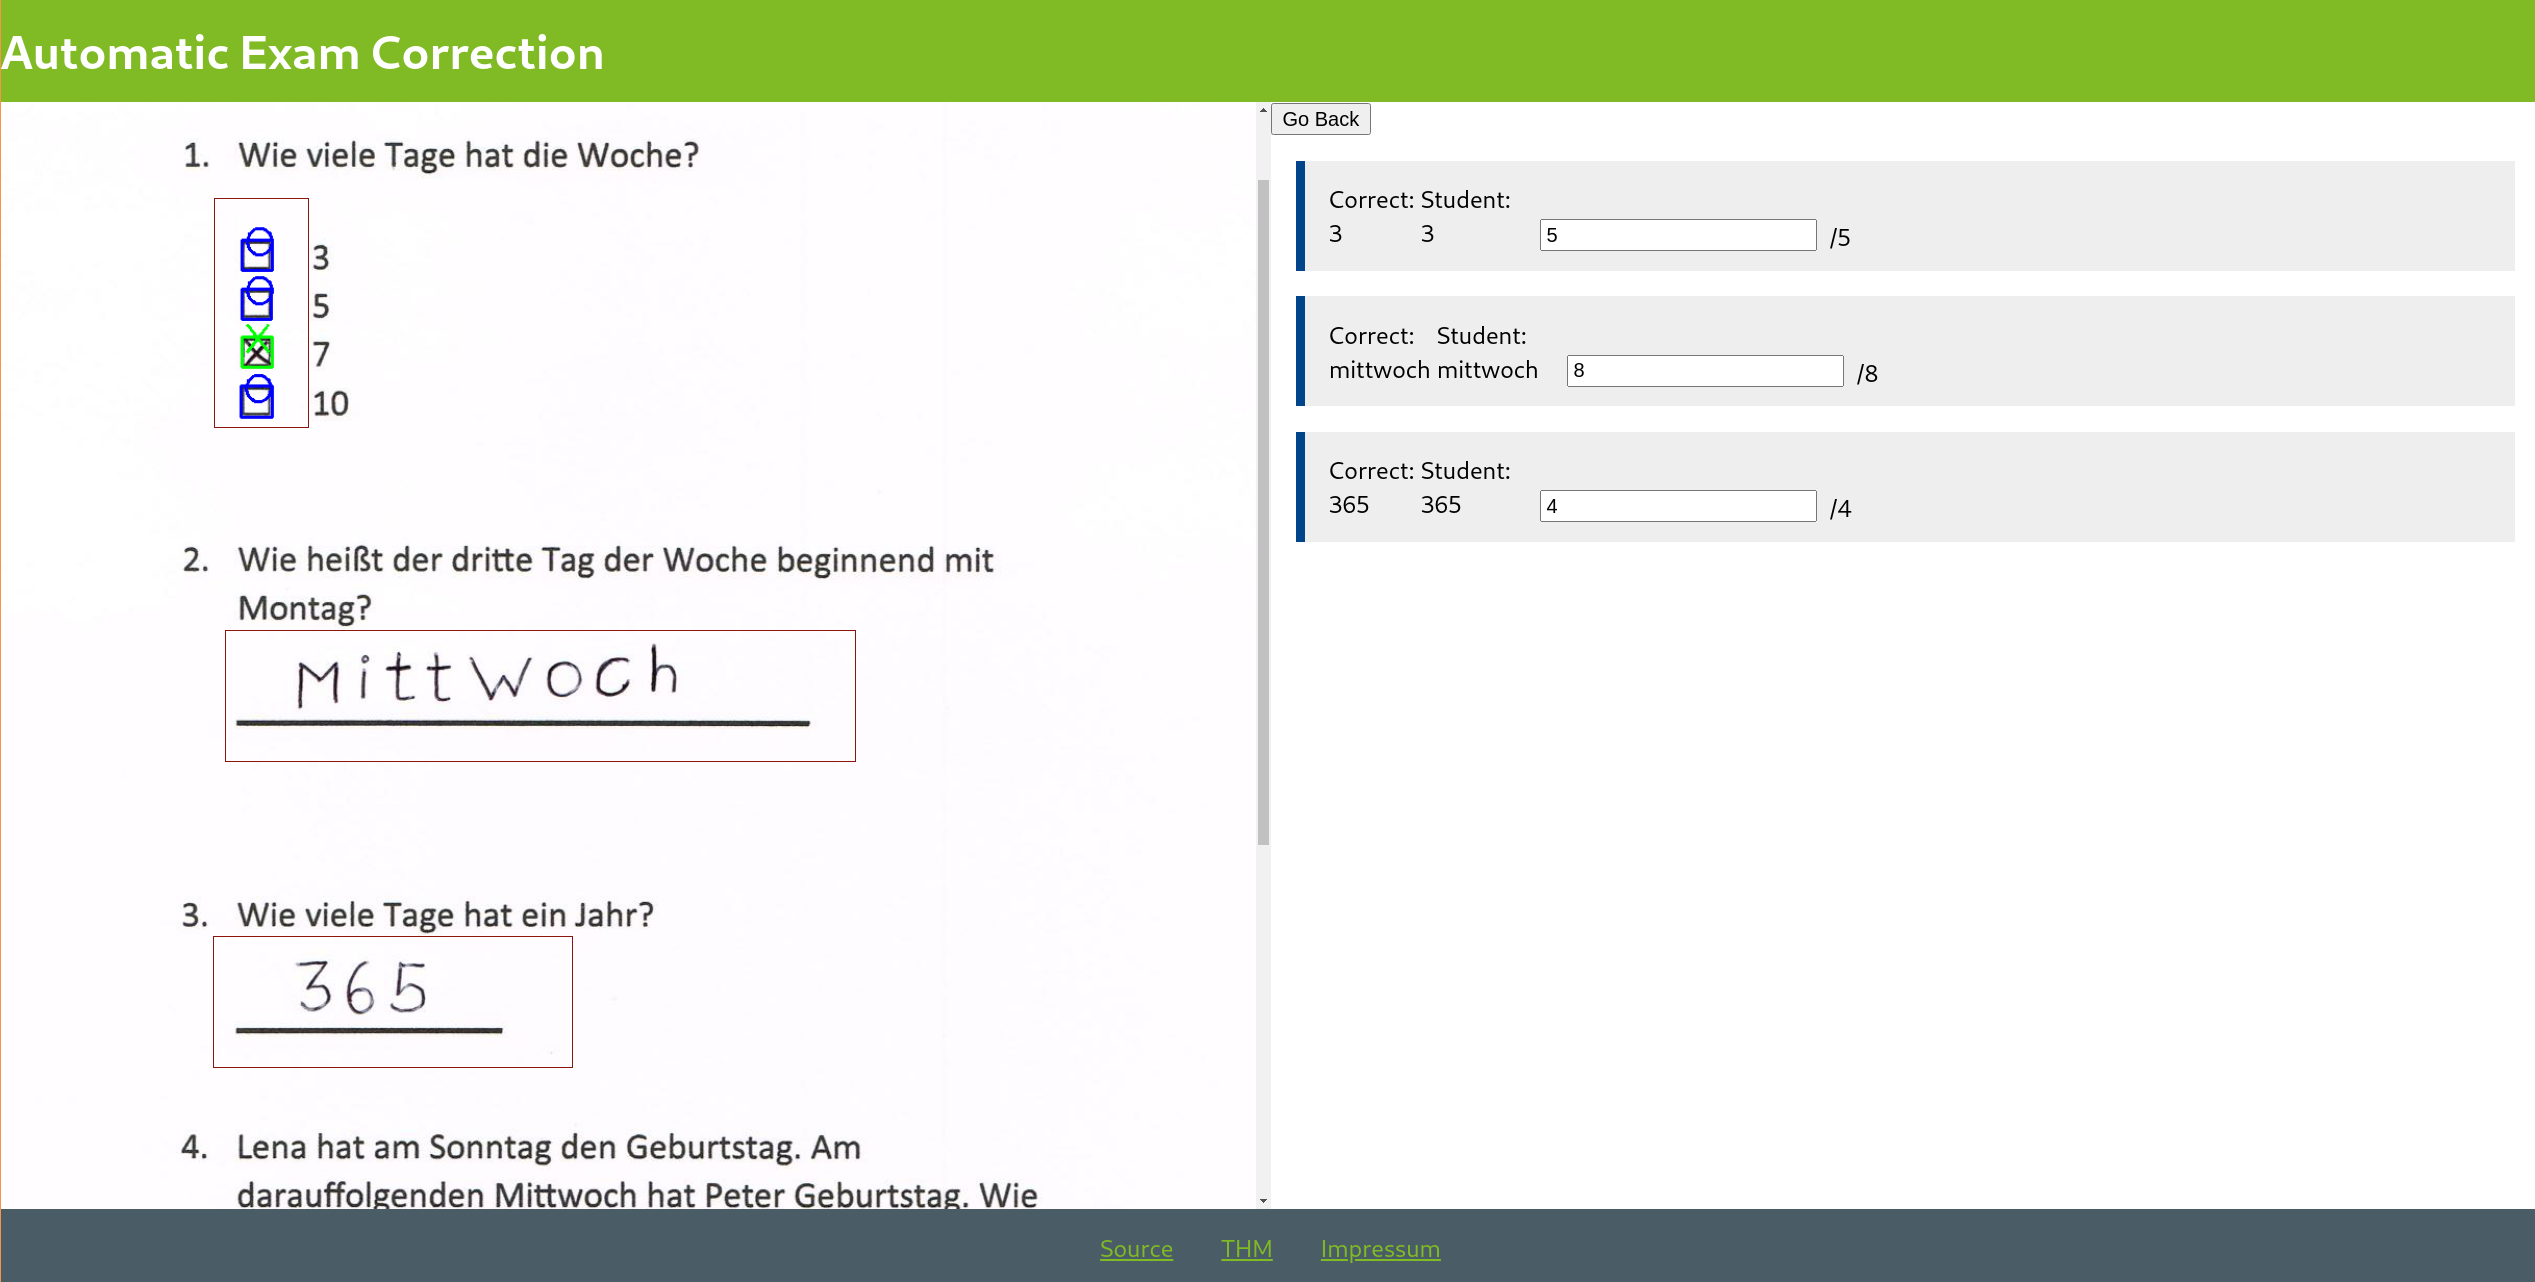
\includegraphics[width=\textwidth]{correct-exam-view}
    \caption{Korrigierte Klausur Ansicht}
\end{figure}

Wenn die Person, welche das Formular ausgef\"ullt hat, Fehler gemacht hat, werden die Punkte auch abgezogen (Aufgabe 3).
Hier kann es zu Fehlern der Software kommen wie in dem folgendem Screenshot sichtbar ist.
Aber sobald in dem Formular die Punkte ge\"andert worden sind, wird das Formular mit der neuen Punktzahl gespeichert.

\begin{figure}[H]
\centering
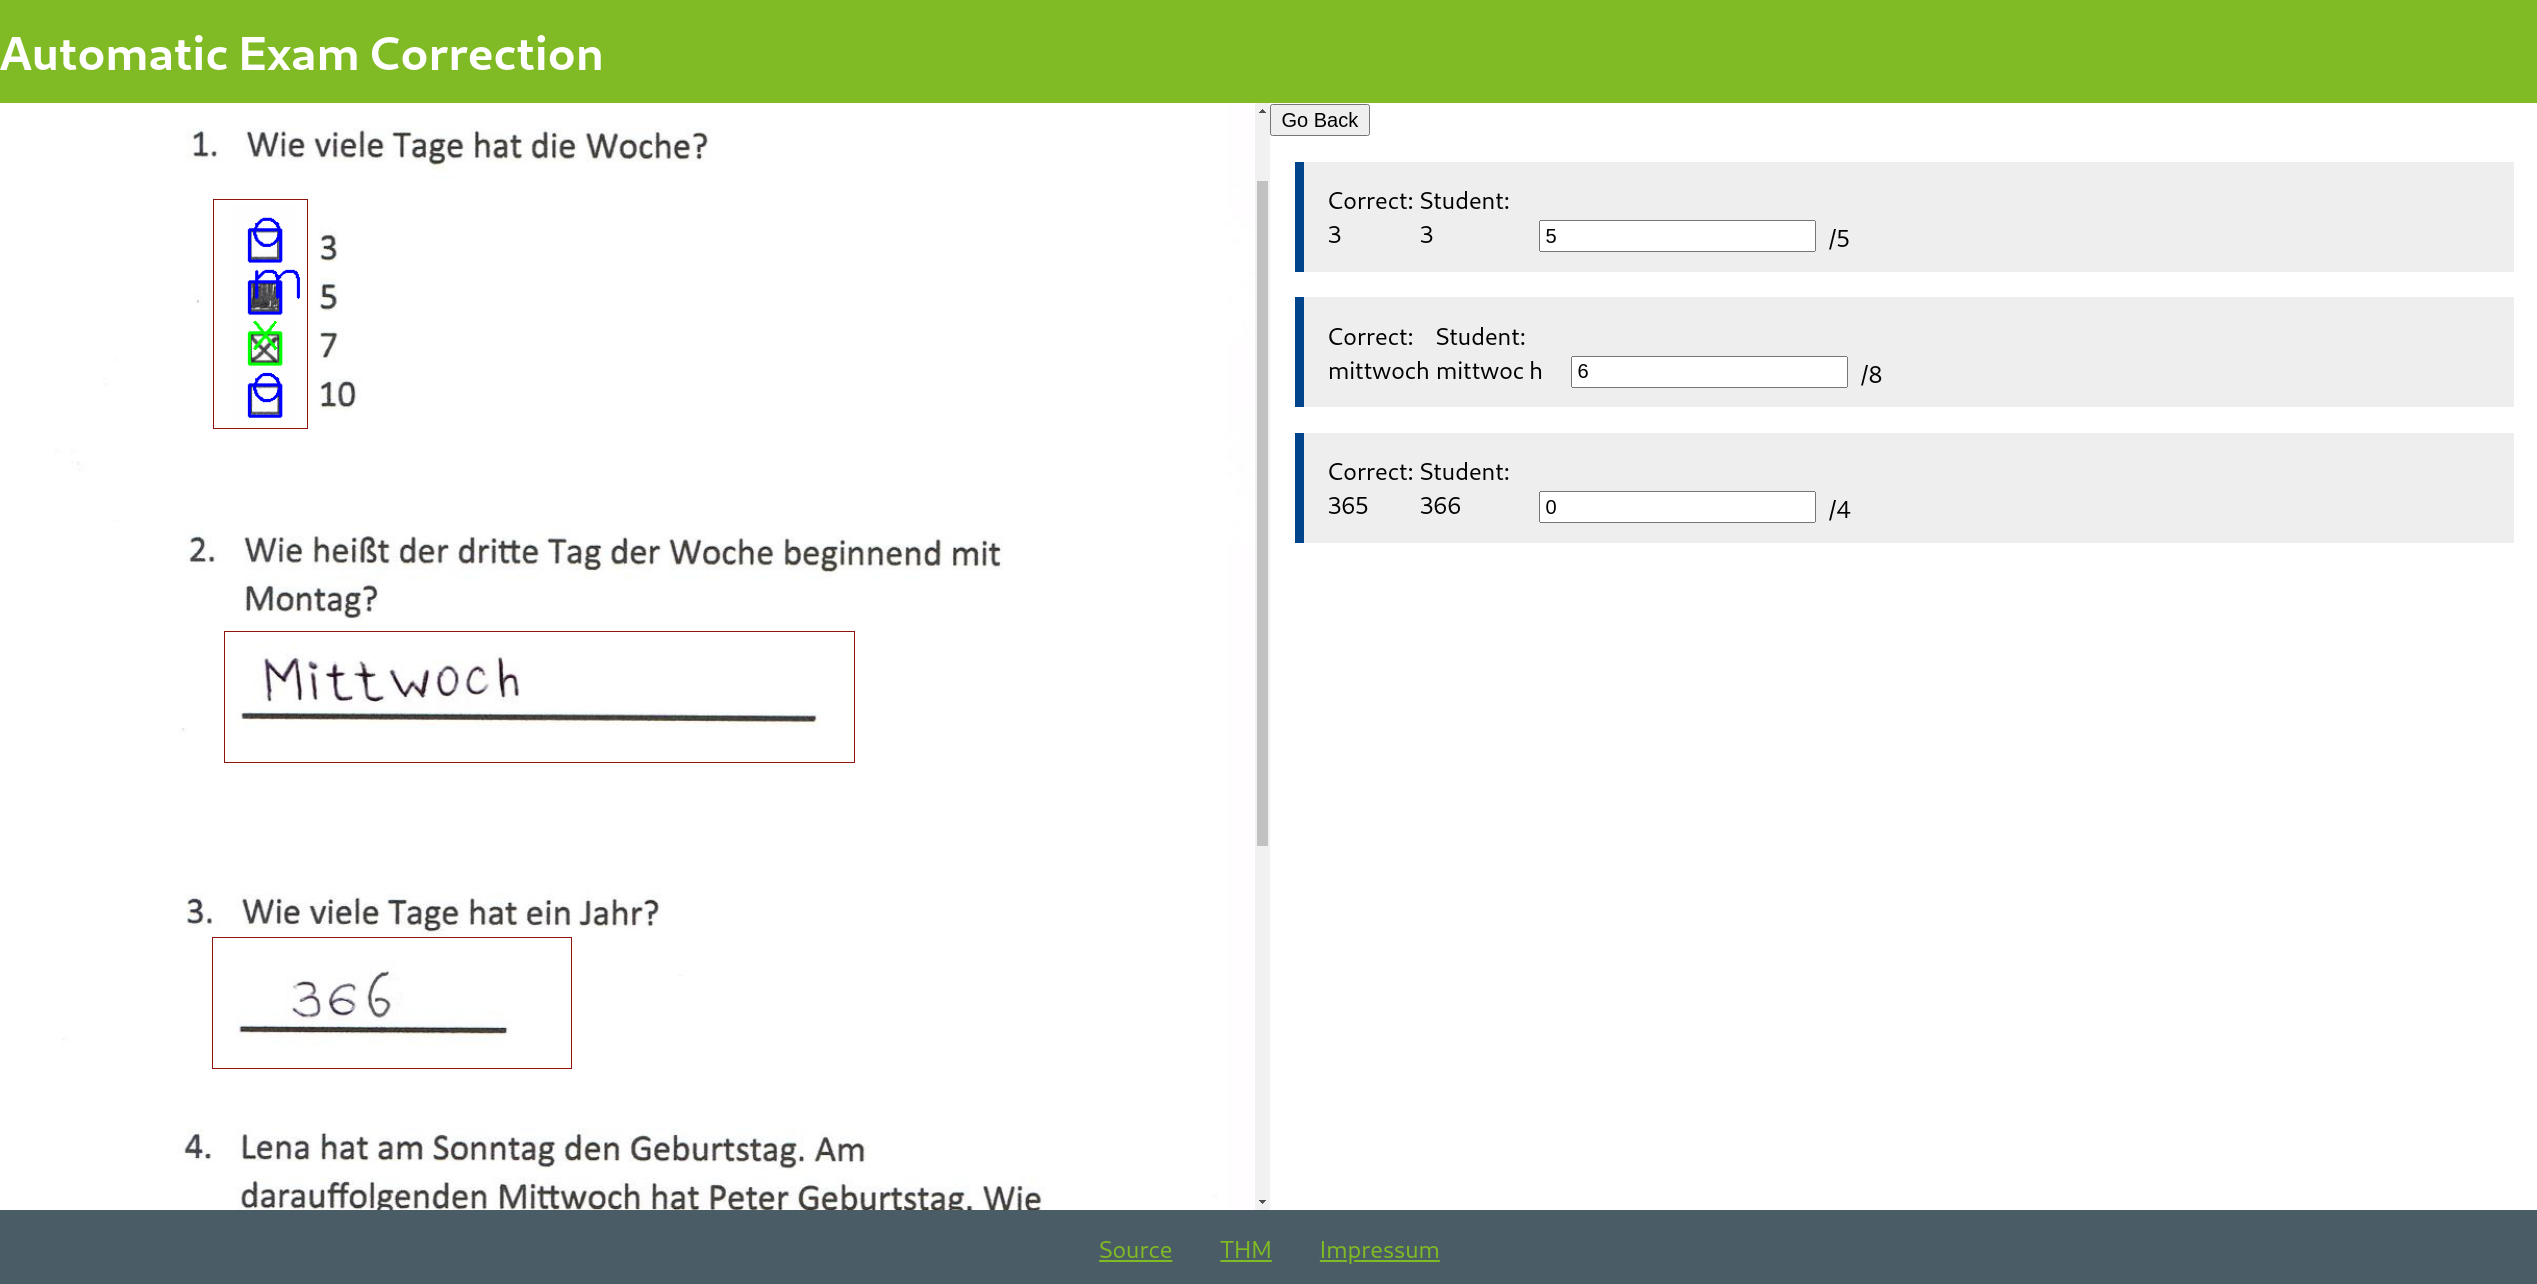
\includegraphics[width=\textwidth]{exam-with-errors}
    \caption{Beispiel mit Fehlern}
\end{figure}

Abschlie{\ss}end kann eine CSV Datei heruntergeladen werden.
CSV Dateien lassen sich leicht in ein Tabellenprogram, wie zum Beispiel Excel, Importieren.
Dabei ist zu beachten, dass der Delimiter (Trennzeichen) der richtigen Sprache entspricht.
\begin{itemize}
    \item{Im Deutschen ist dies ein Semikolon: ';'}
    \item{Im Englischen/Global ist dies ein Komma: ','}
\end{itemize}
